\documentclass[12pt]{extarticle}
\usepackage[utf8]{inputenc}
\usepackage[english,russian]{babel}
\usepackage{vmargin}
\usepackage{indentfirst}
\usepackage[T2A]{fontenc}
\usepackage{graphics}
\usepackage{amsthm}
\usepackage{amsbsy}
\usepackage{amsmath}
\usepackage{amssymb}
\usepackage{amsfonts}
\usepackage{mathtext}
\usepackage[pdftex,a4paper,colorlinks,linkcolor=blue,citecolor=blue]{hyperref}	

\usepackage{mathtext}
\usepackage{mathenv}
\usepackage[pdftex]{graphicx}
\usepackage{array}
\usepackage{graphicx,xcolor}
\usepackage{xcolor}
\usepackage{float}
\usepackage{longtable}

%\parindent = 30pt
%\hoffset = 0pt
%\voffset = 0pt
\oddsidemargin = 100pt
\topmargin = 18pt
%\headheight = 12pt
%\headsep = 25pt
\textheight = 700pt
\textwidth = 440pt
%\marginparsep = 10pt
%\marginparwidth = 103pt

\usepackage{tikz}
\usepackage{verbatim}

\paperwidth = 597pt
\paperheight = 845pt
\numberwithin{equation}{section}

\DeclareMathOperator{\sign}{sign}
\DeclareMathOperator{\const}{const}
\renewcommand{\Re}{\mathop{\mathrm{Re}}\nolimits}
\renewcommand{\Im}{\mathop{\mathrm{Im}}\nolimits}
\newtheorem{algorithm}{Алгоритм}[section]

\begin{document}

\begin{titlepage} \newpage 
\begin{center} МОСКОВСКИЙ ГОСУДАРСТВЕННЫЙ УНИВЕРСИТЕТ ИМ. М.В. ЛОМОНОСОВА\end{center} 
\vspace{8em} \begin{center} 
\Large Механико-математический факультет \\ \end{center}
\vspace{2em} \begin{center} 
\textsc{Отчет по практикуму на ЭВМ \linebreak 
\textbf{Численное моделирование нестационарного одномерного течения газа: \linebreak
Схема для $\log (\rho)$ с центральными разностями}} \end{center}
\vspace{6em} \newbox{\lbox} \savebox{\lbox}{\hbox{Я.Нагорных}} 
\newlength{\maxl} \setlength{\maxl}{\wd\lbox} \hfill\parbox{12	cm}
{ \hspace*{10cm}\hspace*{-5cm}Студент 4 курса:\hfill\hbox to\maxl{Нагорных Я.В.}\\
\hspace*{10cm}\hspace*{-5cm}Преподаватель:\hfill\hbox to\maxl{Попов А.В.}}\\  \vspace{\fill}
\begin{center} Москва \\ 2018\end{center} \end{titlepage}

%\maketitle

%\renewcommand{\contentsname}{Содержание}
\tableofcontents
\renewcommand{\figurename}{График}
\renewcommand{\theequation}{\thesection.\arabic{equation}}


\newpage


\section{Постановка задачи} \label{sec:1-postanovka-zadachi}
Приведем систему уравнений, описывающую нестационарное двумерное движение вязкого баротропного газа:
\begin{equation}
\left\{
	\begin{aligned}
    	&\cfrac{\partial \rho}{\partial t} + \cfrac{\partial \rho u_1}{\partial x_1}+ \cfrac{\partial \rho u_2}{\partial x_2} = 0, \\
	    & 
\cfrac{\partial \rho u_1}{\partial t} + \cfrac{\partial \rho u_1^2}{\partial x_1} + \cfrac{\partial \rho u_1 u_2}{\partial x_2} 
	+ \cfrac{\partial p}{\partial x_1} 
	= \mu \Big(\cfrac{4}{3}\cfrac{\partial^2 u_1}{\partial x_1^2} + \cfrac{\partial^2 u_1}{\partial x_2^2}
	+  \cfrac{1}{3}\cfrac{\partial^2 u_2}{\partial x_1\partial x_2} \Big) + \rho f_1, \\
		&
\cfrac{\partial \rho u_2}{\partial t} + \cfrac{\partial \rho u_1 u_2}{\partial x_1} + \cfrac{\partial \rho u_2^2}{\partial x_2}
	+ \cfrac{\partial p}{\partial x_2} 
	= \mu \Big(\cfrac{1}{3}\cfrac{\partial^2 u_1}{\partial x_1\partial x_2} + \cfrac{\partial^2 u_2}{\partial x_1^2}
	+  \cfrac{4}{3}\cfrac{\partial^2 u_2}{\partial^2 x_2} \Big) + \rho f_2, \\
    	& p = p (\rho).
	\end{aligned}
\right.
\label{eq:1-nachal-zadacha}
\end{equation}
Здесь $\mu$ -- коэффициент вязкости газа (известная неотрицательная константа), $p$ -- давление газа (известная функция), $f$ -- вектор внешних сил (известная функция).

Неизвестные функции $\rho$ и $u$, плотность и скорость соответственно, -- функции от двух переменных $t$ и $x$ (переменные Эйлера), причем $$(t, x) \in Q = [0, T] \times \Omega.$$

В качестве граничных условий берется следующее:
\begin{equation}
\rho|_{\Gamma^-} = \rho_{\gamma} = 1,\quad u_1|_{\Gamma^-} = \omega \in \{0,1;\  1\},\quad \cfrac{\partial u_1}{\partial x_1}\Big|_{\Gamma^+} = 0. \label{eq:1-usl2}
\end{equation}

На оставшейся границе компоненты скорости равны нулю, а функция плотности считается неизвестной.

Для решения задачи введем равномерную сетку $\omega_h$ с шагом $h_x$ по оси $x$, с шагом $h_y$ по оси $y$ и с шагом $\tau$ по оси $t$. 
Введем константы $M_x$, $M_y$ и $N$, такие что $X = M_xh_x$, $Y= M_y h_y$ и $T = N\tau$.

\section{Схема для $\log(\rho)$ с центральными разностями}
\label{scheme1}

Для автоматического обеспечения условия положительности функции плотности систему дифференциальных уравнений можно преобразовать к виду
\begin{equation}
\left\{
\begin{aligned}
& \cfrac{\partial g}{\partial t} + \frac{1}{2}\sum_{k=1}^{2}\left(u_k\cfrac{\partial g}{\partial x_k}+
  \cfrac{\partial u_k g}{\partial x_k} + (2-g)\cfrac{\partial u_k}{\partial x_k}\right) = f_0,\\
& \cfrac{\partial u_k}{\partial t} + \frac{1}{3}(u_k\cfrac{\partial u_k}{\partial x_k} + 
  \cfrac{\partial u_k^2}{\partial x_k})
  + \frac{1}{2}\sum_{m=1,m\neq k}^{2}\left( u_m\cfrac{\partial u_k}{\partial x_m}+
  \cfrac{\partial u_m u_k}{\partial x_m} - u_k\cfrac{\partial u_m}{\partial x_m}\right)
  + p'_{\rho} \cfrac{\partial g}{\partial x_k} = \\
& \qquad\qquad = \cfrac{\mu}{\rho}\left( \frac{4}{3} \cfrac{\partial^2 u_k}{\partial x_k^2} + 
  \sum_{m=1,m\neq k}^{2}\left( \cfrac{\partial^2 u_k}{\partial x_m^2} + 
  \frac{1}{3} \cfrac{\partial^2 u_m}{\partial x_k \partial x_m} \right)\right) + f_k,\qquad k = 1 \dots s,\\
& p = p(\rho), \quad g = \ln \rho.
\end{aligned}
\right.
\end{equation}

Сеточную функцию, разностное приближение для плотности $\rho$, обозначим $H$. 
Аналогично, разностные аналоги $g$ и $u$ обозначим через $G$ и $V$. 
Для поиска численного решения задачи используется следующая разностная схема:
$$\begin{eqnarray}
&\,& G_t + \frac{1}{2} \sum_{k=1}^{2}\left(V_k \hat G_{\stackrel{\circ}{x_k}} + (V_k \hat G)_{\stackrel{\circ}{x_k}} 
  + 2 (\hat V_k)_{\stackrel{\circ}{x_k}} - G(V_k)_{\stackrel{\circ}{x_k}} \right) = f_0,\qquad x \in \Omega _{\bar h};\\
&\,& G_t + \frac{1}{2} \left((V_k \hat G)_{x_k} + 2 (\hat V_k)_{x_k} - G(V_k)_{x_k}\right) -\frac{1}{2}h_k \left( (GV_k)_{x_k\bar x_k}^{+1_k} - \frac{1}{2}(GV_k)_{x_k\bar x_k}^{+2_k} + \right. \nonumber \\
&\,& \qquad\left.  + (2-G)\left((V_k)_{x_k\bar x_k}^{+1_k} - \frac{1}{2} (V_k)_{x_k\bar x_k}^{+2_k}\right)\right) = f_0, \qquad x \in \gamma_k^-,\,\, k = 1,\ 2;\\
&\,& G_t + \frac{1}{2} \left((V_k \hat G)_{\bar x_k} + 2 (\hat V_k)_{\bar x_k} - G(V_k)_{\bar x_k}\right)+ \frac{1}{2}h_k \left( (GV_k)_{x_k\bar x_k}^{-1_k} - \frac{1}{2}(GV_k)_{x_k\bar x_k}^{-2_k} +\right. \nonumber\\
&\,&\qquad \left. + (2-G)\left((V_k)_{x_k\bar x_k}^{-1_k} - \frac{1}{2} (V_k)_{x_k\bar x_k}^{-2_k}\right)\right)  = f_0, \qquad x \in \gamma_k^+,\,\, k = 1,\ 2; \\
&\,& (V_k)_t + \frac{1}{3}\left( V_k(\hat V_k)_{\stackrel{\circ}{x_k}} + (V_k \hat V_k)_{\stackrel{\circ}{x_k}} \right) + \nonumber\\
&\,& \quad + \frac{1}{2}\sum_{m=1,\,m\neq k}^{2}\left(V_m(\hat V_k)_{\stackrel{\circ}{x_m}} + (V_m \hat V_k)_{\stackrel{\circ}{x_m}} - V_k(\hat V_m)_{\stackrel{\circ}{x_m}} \right) + p'_{\rho }(e^{G})\hat G_{\stackrel{\circ}{x_m}} = \nonumber\\
&\,& \qquad = \tilde{\mu} \left( \frac{4}{3}(\hat V_k)_{x_k\bar x_k} + \sum_{m=1,\,m\neq k}^{2}(\hat V_k)_{x_m\bar x_m} \right)- \left(\tilde{\mu} - \mu e^{-G}\right) \times \nonumber\\
&\,&\qquad \quad \times \left( \frac{4}{3}(V_k)_{x_k\bar x_k} + \sum_{m=1,\,m\neq k}^{2}(V_k)_{x_m\bar x_m} \right) + \cfrac{\mu e^{-G}}{3} \sum_{m=1,\,m\neq k}^{2}(V_m)_{\stackrel{\circ}{x_k} \stackrel{\circ}{x_m}} + f_k,\nonumber\\
&\,&\qquad\qquad\qquad\qquad\qquad\qquad\qquad\qquad\qquad\qquad\qquad\qquad\mbox{где } x\in \Omega_{\bar h};\\
&\,& \hat V_k = 0, \qquad x \in \gamma_{\bar h}, \qquad k = 1,\ 2.
\end{eqnarray}$$

Распишем уравнения схемы в поточечном виде и преобразуем их, приведя подобные слагаемые при неизвестных значениях с верхнего слоя. Получим:

\begin{align*}
& 4\cdot G_{m_1,m_2}^{n+1} -\frac{\tau}{h_x} G_{m_1-1,m_2}^{n+1}\left({V_1}_{m_1,m_2}^n + {V_1}_{m_1-1,m_2}^n\right) + \frac{\tau}{h_x} G_{m_1+1,m_2}^{n+1}\left({V_1}_{m_1,m_2}^n + {V_1}_{m_1+1,m_2}^n\right) -\\
& \quad -\frac{\tau}{h_y} G_{m_1,m_2-1}^{n+1}\left({V_2}_{m_1,m_2}^n + {V_2}_{m_1,m_2-1}^n\right) + \frac{\tau}{h_y} G_{m_1,m_2+1}^{n+1}\left({V_2}_{m_1,m_2}^n + {V_2}_{m_1,m_2+1}^n\right) -\\
& \qquad-\frac{2\tau}{h_x} {V_1}_{m_1-1,m_2}^{n+1} + \frac{2\tau}{h_x} {V_1}_{m_1+1,m_2}^{n+1} -\frac{2\tau}{h_y} {V_2}_{m_1,m_2-1}^{n+1} + \frac{2\tau}{h_y} {V_2}_{m_1,m_2+1}^{n+1} = \\
& \qquad\quad =\ 4\cdot G_{m_1,m_2}^n + \tau G_{m_1,m_2}^n 
\left(\cfrac{{V_1}_{m_1+1,m_2}^n - {V_1}_{m_1-1,m_2}^n}{h_x} +  \cfrac{{V_2}_{m_1,m_2+1}^n - {V_2}_{m_1,m_2-1}^n}{h_y}\right) +\ 4\tau f_0, \\
& \qquad\qquad\qquad\qquad\qquad\qquad\qquad\qquad\qquad\qquad\qquad\qquad\qquad\qquad\qquad\qquad\qquad\mbox{где } x\in \Omega _h \\
\end{align*}
\begin{align*}
& G_{0,m_2}^{n+1}\left(2 - \frac{\tau}{h_x}{V_1}_{0,m_2}^n\right) + G_{1,m_2}^{n+1}\frac{\tau}{h_x}{V_1}_{1,m_2}^n + \frac{2\tau}{h_x}{V_1}_{1,m_2}^{n+1} - \frac{2\tau}{h_x}{V_1}_{0,m_2}^{n+1} =  \\
&\quad =  2 \cdot G_{0,m_2}^n + \frac{\tau}{h_x} G_{0,m_2}^n \left({V_1}_{1,m_2}^n - {V_1}_{0,m_2}^n\right) + 2\tau f_0 +\\
& \qquad + \frac{\tau}{h_x} \left( G_{0,m_2}^n {V_1}_{0,m_2}^n - \frac{5}{2}\cdot G_{1,m_2}^n {V_1}_{1,m_2}^n + 2\cdot G_{2,m_2}^n {V_1}_{2,m_2}^n -\right.\\
& \left. \qquad\quad - \frac{1}{2}\cdot G_{3,m_2}^n {V_1}_{3,m_2}^n + \left(2 - G_{0,m_2}^n\right) \cdot \left({V_1}_{0,m_2}^n - 2.5\cdot {V_1}_{1,m_2}^n + 2 {V_1}_{2,m_2}^n - 0.5 {V_1}_{3,m_2}^n\right) \right), \\
& \qquad\qquad\qquad\qquad\qquad\qquad\qquad\qquad\qquad\qquad\qquad\qquad\qquad\qquad\qquad\qquad\qquad\mbox{где } x \in \gamma_k^-
\end{align*}
\begin{align*}
& G_{M,m_2}^{n+1}\left(2 + \frac{\tau}{h_x}{V_1}_{M,m_2}^n\right) - G_{M-1,m_2}^{n+1}\frac{\tau}{h_x}{V_1}_{M-1,m_2}^n + \frac{2\tau}{h_x}{V_1}_{M,m_2}^{n+1} - \frac{2\tau}{h_x}{V_1}_{M-1,m_2}^{n+1} = \\
& \quad=  2\cdot G_{M,m_2}^n + \frac{\tau}{h_x} G_{M,m_2}^n \left({V_1}_{M,m_2}^n - {V_1}_{M-1,m_2}^n\right) + 2\tau f_0 - \frac{\tau}{h_x} \times \Bigg[ G_{M,m_2}^n {V_1}_{M,m_2}^n - \\
&\qquad- \frac{5}{2}\cdot G_{M-1,m_2}^n {V_1}_{M-1,m_2}^n + 2 \cdot G_{M-2,m_2}^n {V_1}_{M-2,m_2}^n - \frac{1}{2}\cdot G_{M-3,m_2}^n {V_1}_{M-3,m_2}^n +\\
&\qquad\quad +\left(2 - G_{M,m_2}^n\right) \cdot \left({V_1}_{M,m_2}^n - \frac{5}{2}\cdot {V_1}_{M-1,m_2}^n + 2 \cdot{V_1}_{M-2,m_2}^n - \frac{1}{2}\cdot  {V_1}_{M-3,m_2}^n\right) \Bigg],\\
& \qquad\qquad\qquad\qquad\qquad\qquad\qquad\qquad\qquad\qquad\qquad\qquad\qquad\qquad\qquad\qquad\qquad\mbox{где } x \in \gamma_k^+
\end{align*}
\begin{align*}
& {V_1}_{m_1,m_2}^{n+1}\left(6 + 4\cdot \tau \tilde{\mu}\left(\cfrac{4}{h_x^2} + \cfrac{3}{h_y^2}\right)\right) + {V_1}_{m_1-1,m_2}^{n+1}\left(-\frac{\tau}{h_x}\left({V_1}_{m_1,m_2}^n + {V_1}_{m_1-1,m_2}^n\right) -\tilde{\mu}\cfrac{8\tau}{h_x^2}\right) +\\
& \quad + {V_1}_{m_1+1,m_2}^{n+1}\left(\frac{\tau}{h_x}\left({V_1}_{m_1,m_2}^n + {V_1}_{m_1+1,m_2}^n\right) -\cfrac{8\tau}{h_x^2}\right) \cdot \tilde{\mu} +\\
& \quad \quad + {V_1}_{m_1,m_2-1}^{n+1}\left(-\frac{3\tau}{2h_y}\left({V_2}_{m_1,m_2}^n + {V_2}_{m_1,m_2-1}^n\right) - \cfrac{6\tau}{h_y^2}\right)\cdot \tilde{\mu}  +\\
& \quad\qquad + {V_1}_{m_1,m_2+1}^{n+1}\left(\frac{3\tau}{2h_y}\left({V_2}_{m_1,m_2}^n + {V_2}_{m_1,m_2+1}^n\right) - \cfrac{6\tau}{h_y^2}\right)\cdot \tilde{\mu}  -\\
& \qquad\qquad- 3\cdot \frac{\tau}{h_x}\cdot p'_{\rho} G_{m_1-1,m_2}^{n+1} + 3\cdot \frac{\tau}{h_x} \cdot p'_{\rho} G_{m_1+1,m_2}^{n+1} = \\
& =  6 \cdot {V_1}_{m_1,m_2}^n + 6 \cdot \tau f_1 + \frac{3}{2}\cdot \frac{\tau}{2h_y}{V_1}_{m_1,m_2}^n \left({V_2}_{m_1,m_2+1}-{V_2}_{m_1,m_2-1}\right) - \\
& \quad - 6\cdot \tau \cdot \left(\tilde{\mu} - \mu e^{-G}\right) \cdot 
  \left(\cfrac{4}{3h_x^2}\left({V_1}_{m_1+1,m_2}^n - 2{V_1}_{m_1,m_2}^n + {V_1}_{m_1-1,m_2}^n\right) \right. \\
&\qquad \left.+  \cfrac{1}{h_y^2}\left({V_1}_{m_1,m_2+1}^n - 2{V_1}_{m_1,m_2}^n + {V_1}_{m_1,m_2-1}^n\right)\right) +\\
& \qquad\quad + \mu e^{-G} \cfrac{\tau}{2h_x h_y}
  \left({V_2}_{m_1+1,m_2+1}^n - {V_2}_{m_1-1,m_2+1}^n - {V_2}_{m_1+1,m_2-1}^n + {V_2}_{m_1-1,m_2-1}^n\right), \\
& \qquad\qquad\qquad\qquad\qquad\qquad\qquad\qquad\qquad\qquad\qquad\qquad\qquad\qquad\qquad\mbox{где } \tilde{\mu} = \mu \|e^{-G}\|.
\end{align*}

%\include{./2_scheme_formula}
%\section{Тестирование}

\subsection{$\mu=0.1$}
\begin{center}
\begin{tabular}{||c|c|c|c||}
\hline
\hline
\multicolumn{4}{||c||}{$\|g-G\| _{C}$}\\ 
\hline
\hline
$\tau \backslash h$ & 1.00000 & 0.50000 & 0.25000\\ 
\hline
0.500& 3.191555e-01 &2.247489e-01 &2.243865e-01 \\
\hline
0.250& 3.043471e-01 &1.629398e-01 &1.491416e-01 \\
\hline
0.125& 2.876430e-01 &1.187079e-01 &9.785144e-02 \\
\hline
\hline
\end{tabular}
\end{center}
\begin{center}
\begin{tabular}{||c|c|c|c||}
\hline
\hline
\multicolumn{4}{||c||}{$\|g-G\| _{L_2}$}\\ 
\hline
\hline
$\tau \backslash h$ & 1.00000 & 0.50000 & 0.25000\\ 
\hline
0.500& 9.512504e-01 &8.355700e-01 &8.204384e-01 \\ 
\hline
0.250& 6.122799e-01 &4.612271e-01 &4.428729e-01 \\
\hline
0.125& 4.495678e-01 &2.581024e-01 &2.352407e-01 \\
\hline
\hline
\end{tabular}
\end{center}
\begin{center}
\begin{tabular}{||c|c|c|c||}
\hline
\hline
\multicolumn{4}{||c||}{$\|g-G\| _{v_2^1}$}\\ 
\hline
\hline
$\tau \backslash h$ & 1.00000 & 0.50000 & 0.25000\\ 
\hline 
0.500& 1.385544e+00 &1.114565e+00 &9.792058e-01 \\ 
\hline
0.250& 1.210866e+00 &8.926209e-01 &7.084297e-01 \\ 
\hline
0.125& 1.155027e+00 &8.174585e-01 &6.073713e-01 \\ 
\hline
\hline
\end{tabular}
\end{center}
\begin{center}
\begin{tabular}{||c|c|c|c||}
\hline
\hline
\multicolumn{4}{||c||}{$\|u_1-V_1\| _{C}$}\\ 
\hline
\hline
$\tau \backslash h$ & 1.00000 & 0.50000 & 0.25000\\ 
\hline 
0.500& 3.979879e-01 &3.622549e-01 &3.583263e-01 \\ 
\hline
0.250& 2.643974e-01 &2.274248e-01 &2.187875e-01 \\ 
\hline
0.125& 2.065245e-01 &1.377734e-01 &1.260013e-01 \\ 
\hline
\hline
\end{tabular}
\end{center}
\begin{center}
\begin{tabular}{||c|c|c|c||}
\hline
\hline
\multicolumn{4}{||c||}{$\|u_1-V_1\| _{L_2}$}\\ 
\hline
\hline
$\tau \backslash h$ & 1.00000 & 0.50000 & 0.25000\\ 
\hline 
0.500& 1.149149e+00 &1.132800e+00 &1.131374e+00 \\ 
\hline
0.250& 6.822144e-01 &6.370385e-01 &6.334057e-01 \\ 
\hline
0.125& 4.361231e-01 &3.451439e-01 &3.385633e-01 \\ 
\hline
\hline
\end{tabular}
\end{center}
\begin{center}
\begin{tabular}{||c|c|c|c||}
\hline
\hline
\multicolumn{4}{||c||}{$\|u_1-V_1\| _{v_2^1}$}\\ 
\hline
\hline
$\tau \backslash h$ & 1.00000 & 0.50000 & 0.25000\\ 
\hline 
0.500& 4.621676e+00 &3.323153e+00 &2.462723e+00 \\ 
\hline
0.250& 4.690418e+00 &3.298016e+00 &2.352245e+00 \\ 
\hline
0.125& 4.759038e+00 &3.321124e+00 &2.336537e+00 \\ 
\hline
\hline
\end{tabular}
\end{center}
\begin{center}
\begin{tabular}{||c|c|c|c||}
\hline
\hline
\multicolumn{4}{||c||}{$\|u_2- V_2\| _{C}$}\\ 
\hline
\hline
$\tau \backslash h$ & 1.00000 & 0.50000 & 0.25000\\ 
\hline 
0.500& 1.544142e-01 &1.391937e-01 &1.379958e-01 \\ 
\hline
0.250& 1.151507e-01 &8.370939e-02 &8.120909e-02 \\ 
\hline
0.125& 9.038622e-02 &4.830719e-02 &4.470352e-02 \\ 
\hline
\hline
\end{tabular}
\end{center}
\begin{center}
\begin{tabular}{||c|c|c|c||}
\hline
\hline
\multicolumn{4}{||c||}{$\|u_2-V_2\| _{L_2}$}\\ 
\hline
\hline
$\tau \backslash h$ & 1.00000 & 0.50000 & 0.25000\\ 
\hline 
0.500& 5.098528e-01 &4.514006e-01 &4.401044e-01 \\ 
\hline
0.250& 3.377369e-01 &2.619125e-01 &2.484032e-01 \\ 
\hline
0.125& 2.432280e-01 &1.504754e-01 &1.349097e-01 \\ 
\hline
\hline
\end{tabular}
\end{center}
\begin{center}
\begin{tabular}{||c|c|c|c||}
\hline
\hline
\multicolumn{4}{||c||}{$\|u_2-V_2\| _{v_2^1}$}\\ 
\hline
\hline
$\tau \backslash h$ & 1.00000 & 0.50000 & 0.25000\\ 
\hline 
0.500& 9.951011e-01 &7.361388e-01 &5.979325e-01 \\ 
\hline
0.250& 8.503144e-01 &5.894178e-01 &4.431625e-01 \\ 
\hline
0.125& 7.775693e-01 &5.189529e-01 &3.699671e-01 \\ 
\hline
\hline
\end{tabular}
\end{center}
\subsection{$\mu=0.01$}       
\begin{center}
\begin{tabular}{||c|c|c|c||}
\hline
\hline
\multicolumn{4}{||c||}{$\|g-G\| _{C}$}\\ 
\hline
\hline
$\tau \backslash h$ & 1.00000 & 0.50000 & 0.25000\\ 
\hline 
0.500& 3.332275e-01 &2.317920e-01 &2.308903e-01 \\ 
\hline
0.250& 3.227055e-01 &1.738487e-01 &1.583301e-01 \\ 
\hline
0.125& 3.101889e-01 &1.297109e-01 &1.059268e-01 \\ 
\hline
\hline
\hline
\end{tabular}
\end{center}
\begin{center}
\begin{tabular}{||c|c|c|c||}
\hline
\hline
\multicolumn{4}{||c||}{$\|g-G\| _{L_2}$}\\ 
\hline
\hline
$\tau \backslash h$ & 1.00000 & 0.50000 & 0.25000\\ 
\hline 
0.500& 9.769827e-01 &8.604924e-01 &8.452480e-01 \\ 
\hline
0.250& 6.319185e-01 &4.775693e-01 &4.588406e-01 \\ 
\hline
0.125& 4.690277e-01 &2.688623e-01 &2.448913e-01 \\ 
\hline
\hline
\end{tabular}
\end{center}
\begin{center}
\begin{tabular}{||c|c|c|c||}
\hline
\hline
\multicolumn{4}{||c||}{$\|g-G\| _{v_2^1}$}\\ 
\hline
$\tau \backslash h$ & 1.00000 & 0.50000 & 0.25000\\ 
\hline
\hline 
0.500& 1.404438e+00 &1.133190e+00 &9.999392e-01 \\ 
\hline
0.250& 1.224002e+00 &9.019652e-01 &7.190158e-01 \\ 
\hline
0.125& 1.168566e+00 &8.230314e-01 &6.124281e-01 \\ 
\hline
\hline
\end{tabular}
\end{center}
\begin{center}
\begin{tabular}{||c|c|c|c||}
\hline
\hline
\multicolumn{4}{||c||}{$\|u_1-V_1\| _{C}$}\\ 
\hline
\hline
$\tau \backslash h$ & 1.00000 & 0.50000 & 0.25000\\ 
\hline 
0.500& 4.081024e-01 &3.697396e-01 &3.661379e-01 \\ 
\hline
0.250& 2.740035e-01 &2.351150e-01 &2.260646e-01 \\ 
\hline
0.125& 2.252334e-01 &1.456298e-01 &1.317880e-01 \\ 
\hline
\hline
\end{tabular}
\end{center}
\begin{center}
\begin{tabular}{||c|c|c|c||}
\hline
\hline
\multicolumn{4}{||c||}{$\|u_1-V_1\| _{L_2}$}\\ 
\hline
\hline
$\tau \backslash h$ & 1.00000 & 0.50000 & 0.25000\\ 
\hline 
0.500& 1.200346e+00 &1.181441e+00 &1.179247e+00 \\ 
\hline
0.250& 7.210320e-01 &6.706195e-01 &6.656928e-01 \\ 
\hline
0.125& 4.662389e-01 &3.667748e-01 &3.583753e-01 \\ 
\hline
\hline
\end{tabular}
\end{center}
\begin{center}
\begin{tabular}{||c|c|c|c||}
\hline
\hline
\multicolumn{4}{||c||}{$\|u_1-V_1\| _{v_2^1}$}\\ 
\hline
\hline
$\tau \backslash h$ & 1.00000 & 0.50000 & 0.25000\\ 
\hline 
0.500& 4.620662e+00 &3.331493e+00 &2.479650e+00 \\ 
\hline
0.250& 4.682651e+00 &3.296842e+00 &2.356233e+00 \\ 
\hline
0.125& 4.750031e+00 &3.317148e+00 &2.335832e+00 \\ 
\hline
\hline
\end{tabular}
\end{center}
\begin{center}
\begin{tabular}{||c|c|c|c||}
\hline
\hline
\multicolumn{4}{||c||}{$\|u_2-V_2\| _{C}$}\\ 
\hline
\hline
$\tau \backslash h$ & 1.00000 & 0.50000 & 0.25000\\ 
\hline 
0.500& 1.651374e-01 &1.502980e-01 &1.491544e-01 \\ 
\hline
0.250& 1.226988e-01 &9.135306e-02 &8.934564e-02 \\ 
\hline
0.125& 9.669605e-02 &5.290997e-02 &4.973908e-02 \\ 
\hline
\hline
\end{tabular}
\end{center}
\begin{center}
\begin{tabular}{||c|c|c|c||}
\hline
\hline
\multicolumn{4}{||c||}{$\|u_2-V_2\| _{L_2}$}\\ 
\hline
\hline
$\tau \backslash h$ & 1.00000 & 0.50000 & 0.25000\\ 
\hline 
0.500& 5.296704e-01 &4.727790e-01 &4.619251e-01 \\ 
\hline
0.250& 3.525451e-01 &2.763621e-01 &2.631604e-01 \\ 
\hline
0.125& 2.552148e-01 &1.592887e-01 &1.438254e-01 \\ 
\hline
\hline
\end{tabular}
\end{center}
\begin{center}
\begin{tabular}{||c|c|c|c||}
\hline
\hline
\multicolumn{4}{||c||}{$\|u_2-V_2\| _{v_2^1}$}\\ 
\hline
\hline
$\tau \backslash h$ & 1.00000 & 0.50000 & 0.25000\\ 
\hline 
0.500& 1.007894e+00 &7.515347e-01 &6.155485e-01 \\ 
\hline
0.250& 8.573573e-01 &5.973214e-01 &4.526872e-01 \\ 
\hline
0.125& 7.812806e-01 &5.219918e-01 &3.738559e-01 \\ 
\hline
\hline
\end{tabular}
\end{center}

\subsection{$\mu=0.001$}   
\begin{center}
\begin{tabular}{||c|c|c|c||}
\hline
\hline
\multicolumn{4}{||c||}{$\|g-G\| _{C}$}\\
\hline
\hline
$\tau \backslash h$ & 1.00000 & 0.50000 & 0.25000\\ 
\hline 
0.500& 3.346899e-01 &2.325533e-01 &2.315276e-01 \\
\hline
0.250& 3.246620e-01 &1.750017e-01 &1.592995e-01 \\ 
\hline
0.125& 3.126662e-01 &1.309073e-01 &1.068023e-01 \\ 
\hline
\hline
\end{tabular}
\end{center}
\begin{center}
\begin{tabular}{||c|c|c|c||}
\hline
\hline
\multicolumn{4}{||c||}{$\|g-G\| _{L_2}$}\\ 
\hline
\hline 
$\tau \backslash h$ & 1.00000 & 0.50000 & 0.25000\\ 
\hline 
0.500& 9.796632e-01 &8.630954e-01 &8.478420e-01 \\
\hline
0.250& 6.340402e-01 &4.792887e-01 &4.605218e-01 \\ 
\hline
0.125& 4.714032e-01 &2.700253e-01 &2.459161e-01 \\ 
\hline
\hline
\end{tabular}
\end{center}
\begin{center}
\begin{tabular}{||c|c|c|c||}
\hline
\hline
\multicolumn{4}{||c||}{$\|g-G\| _{v_2^1}$}\\ 
\hline 
\hline
$\tau \backslash h$ & 1.00000 & 0.50000 & 0.25000\\ 
\hline 
0.500& 1.406413e+00 &1.135145e+00 &1.002115e+00 \\
\hline
0.250& 1.225423e+00 &9.029572e-01 &7.201406e-01 \\ 
\hline
0.125& 1.170173e+00 &8.236647e-01 &6.129941e-01 \\ 
\hline
\hline
\end{tabular}
\end{center}
\begin{center}
\begin{tabular}{||c|c|c|c||}
\hline
\hline
\multicolumn{4}{||c||}{$\|u_1-V_1\| _{C}$}\\ 
\hline
\hline
$\tau \backslash h$ & 1.00000 & 0.50000 & 0.25000\\ 
\hline 
0.500& 4.091439e-01 &3.705469e-01 &3.669681e-01 \\
\hline
0.250& 2.750049e-01 &2.359130e-01 &2.268182e-01 \\ 
\hline
0.125& 2.273044e-01 &1.464708e-01 &1.323957e-01 \\ 
\hline
\hline
\end{tabular}
\end{center}
\begin{center}
\begin{tabular}{||c|c|c|c||}
\hline
\hline
\multicolumn{4}{||c||}{$\|u_1-V_1\| _{L_2}$}\\ 
\hline
\hline 
$\tau \backslash h$ & 1.00000 & 0.50000 & 0.25000\\ 
\hline 
0.500& 1.205739e+00 &1.186552e+00 &1.184275e+00 \\
\hline
0.250& 7.252048e-01 &6.741907e-01 &6.691166e-01 \\ 
\hline
0.125& 4.695859e-01 &3.691123e-01 &3.604995e-01 \\ 
\hline
\hline
\end{tabular}
\end{center}
\begin{center}
\begin{tabular}{||c|c|c|c||}
\hline
\hline
\multicolumn{4}{||c||}{$\|u_1-V_1\| _{v_2^1}$}\\ 
\hline
\hline
$\tau \backslash h$ & 1.00000 & 0.50000 & 0.25000\\ 
\hline 
0.500& 4.620623e+00 &3.332436e+00 &2.481492e+00 \\
\hline
0.250& 4.681850e+00 &3.296748e+00 &2.356691e+00 \\ 
\hline
0.125& 4.749051e+00 &3.316714e+00 &2.335765e+00 \\ 
\hline
\hline
\end{tabular}
\end{center}
\begin{center}
\begin{tabular}{||c|c|c|c||}
\hline
\hline
\multicolumn{4}{||c||}{$\|u_2-V_2\| _{C}$}\\ 
\hline
\hline 
$\tau \backslash h$ & 1.00000 & 0.50000 & 0.25000\\ 
\hline 
1.662841e-01 &1.514788e-01 &1.503662e-01 \\
\hline
1.234986e-01 &9.217657e-02 &9.022623e-02 \\ 
\hline
9.738230e-02 &5.341048e-02 &5.029295e-02 \\ 
\hline
\hline
\end{tabular}
\end{center}
\begin{center}
\begin{tabular}{||c|c|c|c||}
\hline
\hline
\multicolumn{4}{||c||}{$\|u_2-V_2\| _{L_2}$}\\ 
\hline
\hline
$\tau \backslash h$ & 1.00000 & 0.50000 & 0.25000\\ 
\hline 
0.500& 5.318001e-01 &4.750835e-01 &4.642791e-01 \\ 
\hline
0.250& 3.541905e-01 &2.779583e-01 &2.647925e-01 \\ 
\hline
0.125& 2.566181e-01 &1.602784e-01 &1.448298e-01 \\ 
\hline
\hline
\end{tabular}
\end{center}
\begin{center}
\begin{tabular}{||c|c|c|c||}
\hline
\hline
\multicolumn{4}{||c||}{$\|u_2-V_2\| _{v_2^1}$}\\ 
\hline
\hline
$\tau \backslash h$ & 1.00000 & 0.50000 & 0.25000\\ 
\hline 
0.500& 1.009266e+00 &7.531993e-01 &6.174574e-01 \\ 
\hline
0.250& 8.581391e-01 &5.981973e-01 &4.537501e-01 \\ 
\hline
0.125& 7.817225e-01 &5.223316e-01 &3.742988e-01 \\ 
\hline
\hline
\end{tabular}
\end{center}
%\section{Рассчет для неизвестного решения}

\subsection{Графики для $\mu=0.1$} 
\subsubsection{$M_x=10$; $M_y=10$; $T=10$}
\begin{figure}[H]
\begin{minipage}[h]{0.43\linewidth}
\center{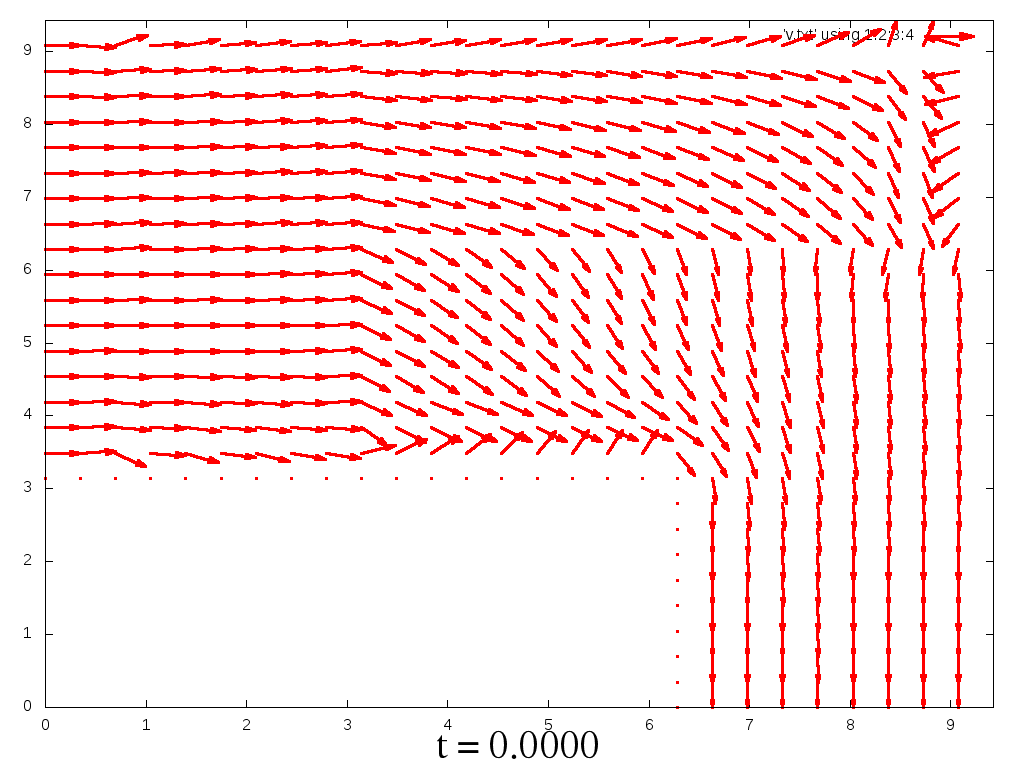
\includegraphics[width=1\linewidth]{./pics/0.1-10-10-21/v/0.png}}
\end{minipage}
\hfill
\begin{minipage}[h]{0.43\linewidth}
\center{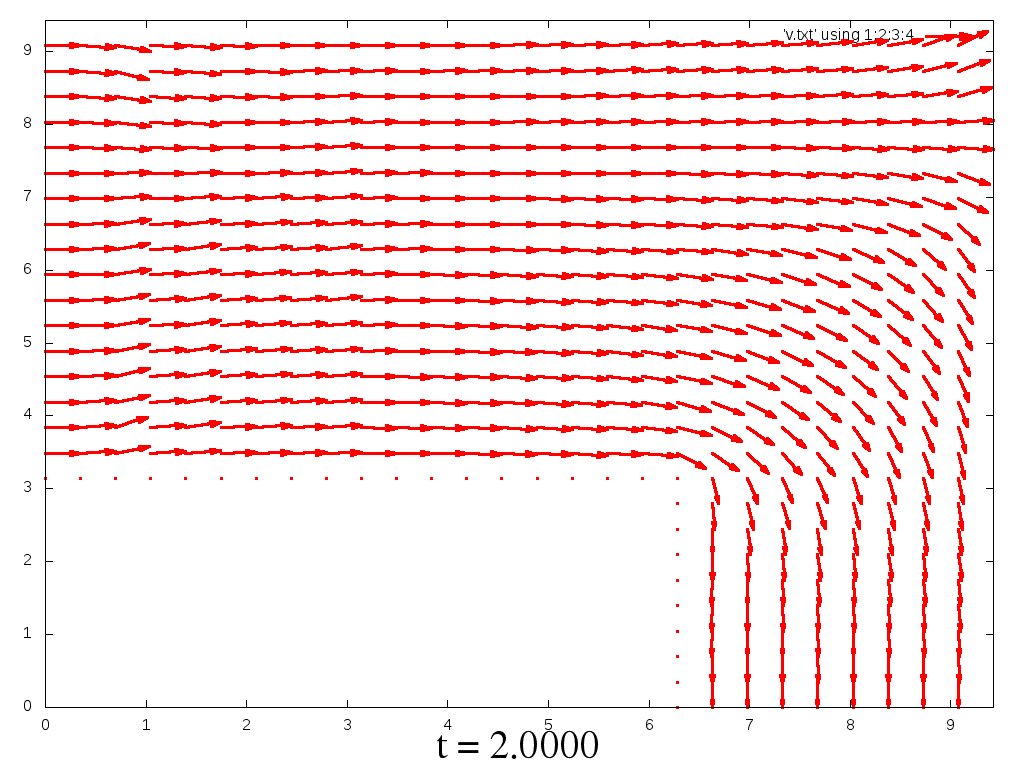
\includegraphics[width=1\linewidth]{./pics/0.1-10-10-21/v/4.png}}
\end{minipage}
\end{figure}

\begin{figure}[H]
\begin{minipage}[h]{0.43\linewidth}
\center{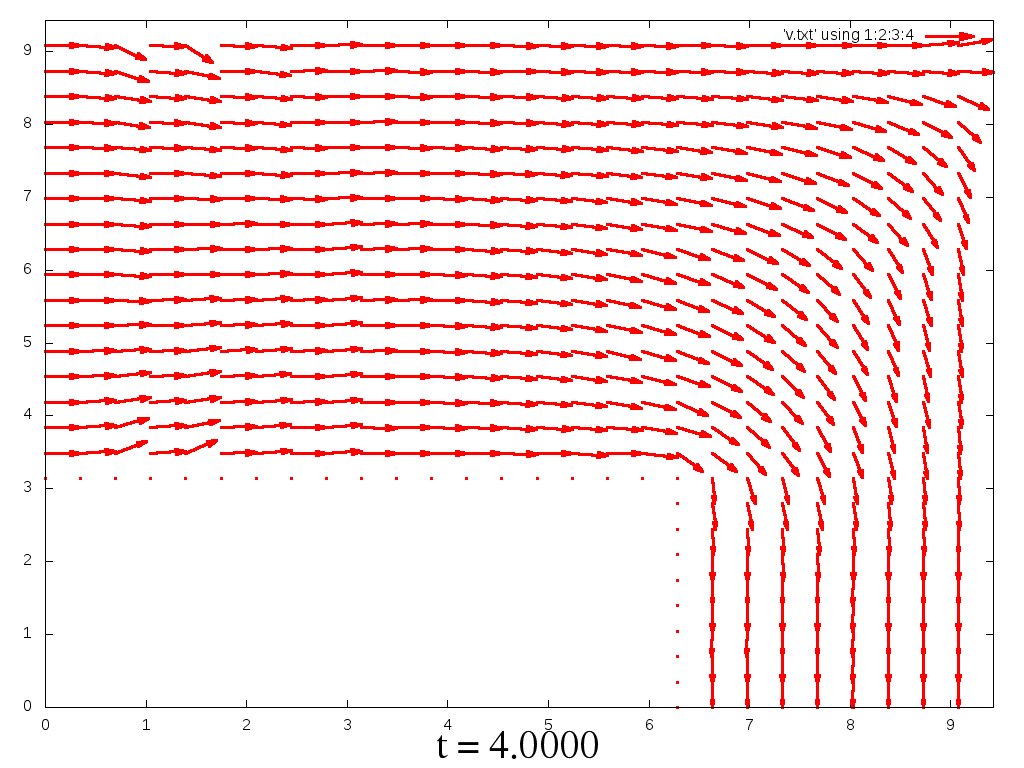
\includegraphics[width=1\linewidth]{./pics/0.1-10-10-21/v/8.png}}
\end{minipage}
\hfill
\begin{minipage}[h]{0.43\linewidth}
\center{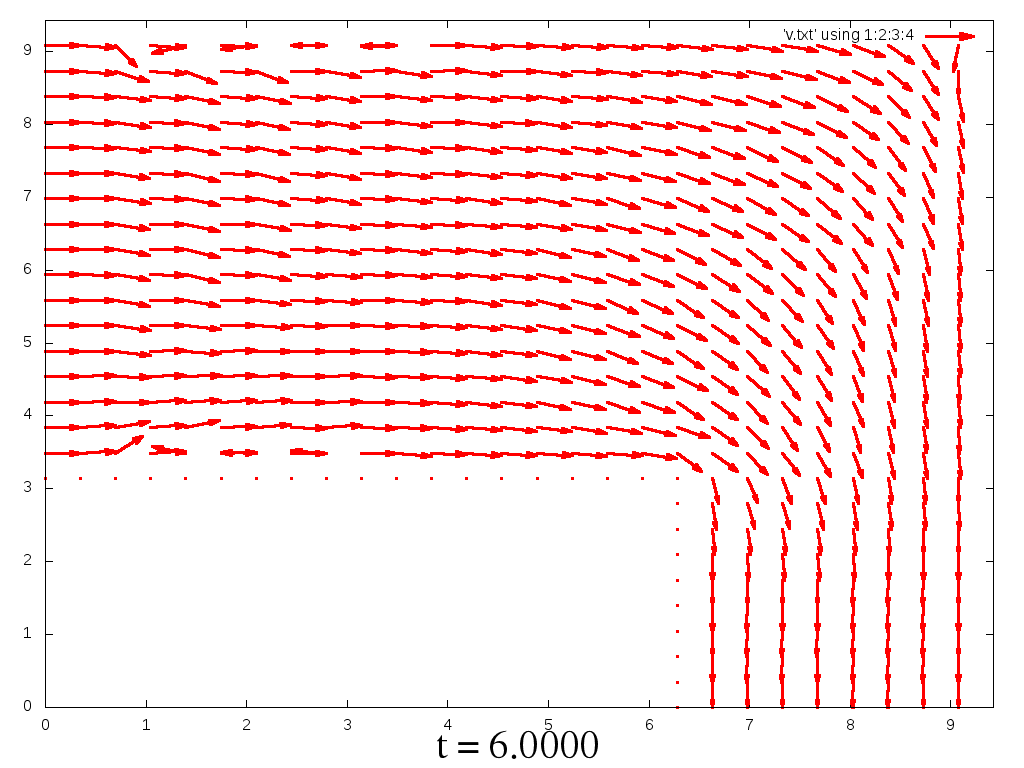
\includegraphics[width=1\linewidth]{./pics/0.1-10-10-21/v/12.png}}
\end{minipage}
\end{figure}

\begin{figure}[H]
\begin{minipage}[h]{0.43\linewidth}
\center{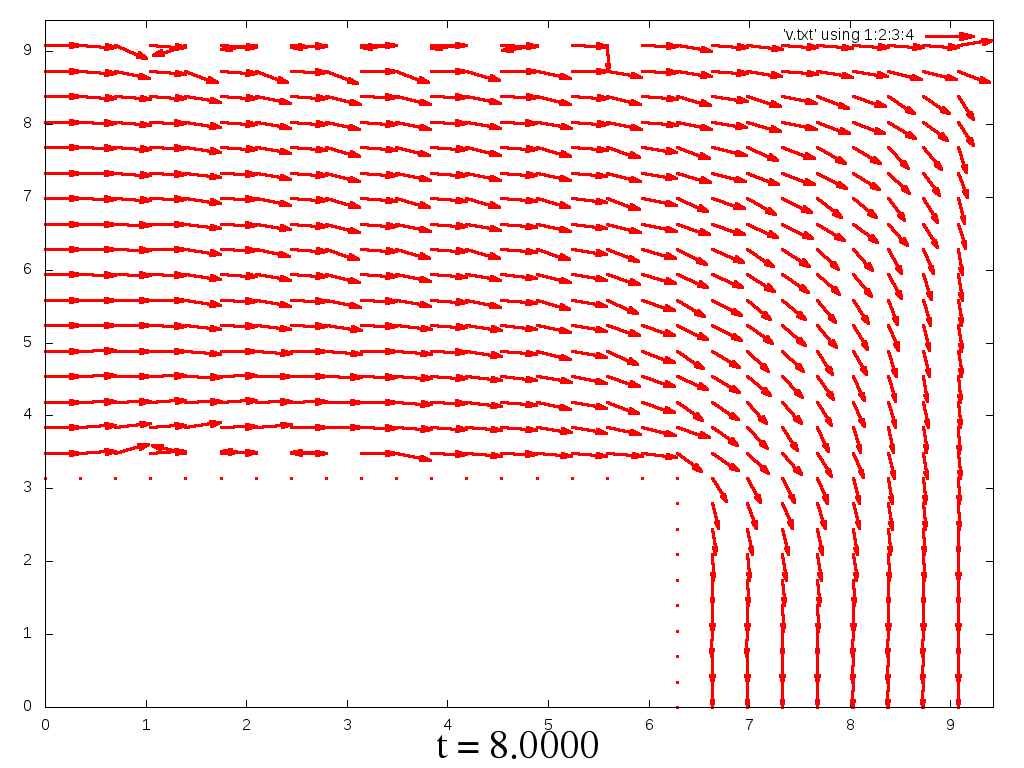
\includegraphics[width=1\linewidth]{./pics/0.1-10-10-21/v/16.png}}
\end{minipage}
\hfill
\begin{minipage}[h]{0.43\linewidth}
\center{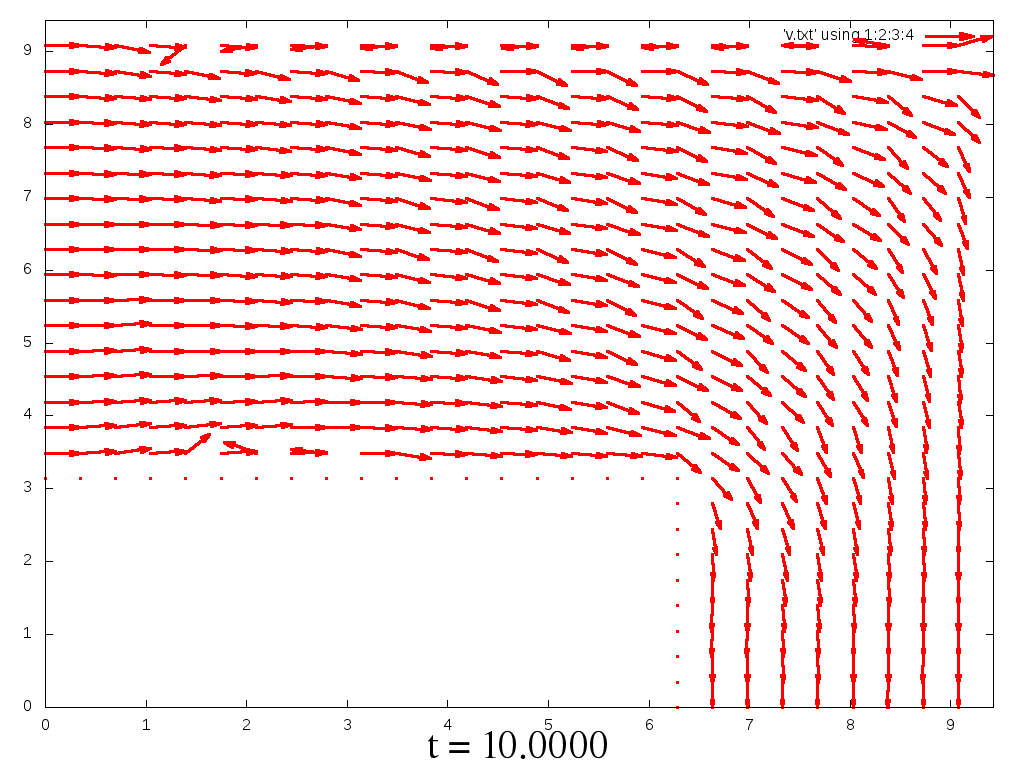
\includegraphics[width=1\linewidth]{./pics/0.1-10-10-21/v/20.png}}
\end{minipage}
\end{figure}

\begin{figure}[H]
\begin{minipage}[h]{0.43\linewidth}
\center{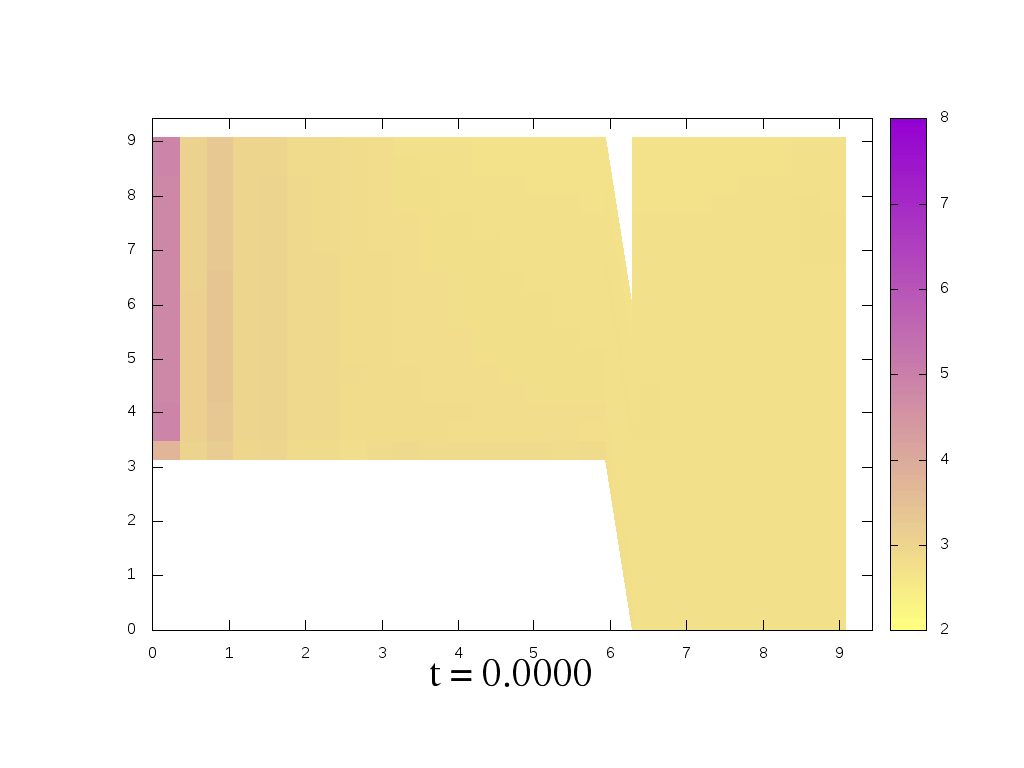
\includegraphics[width=1\linewidth]{./pics/0.1-10-10-21/g/0.png}}
\end{minipage}
\hfill
\begin{minipage}[h]{0.43\linewidth}
\center{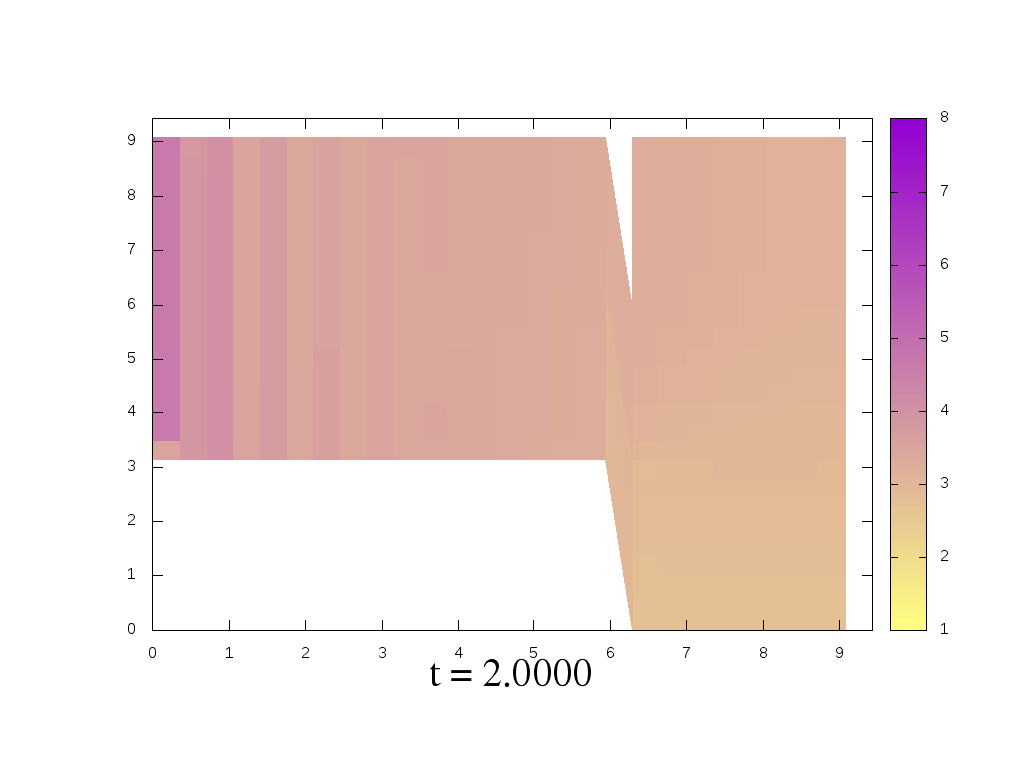
\includegraphics[width=1\linewidth]{./pics/0.1-10-10-21/g/4.png}}
\end{minipage}
\end{figure}

\begin{figure}[H]
\begin{minipage}[h]{0.43\linewidth}
\center{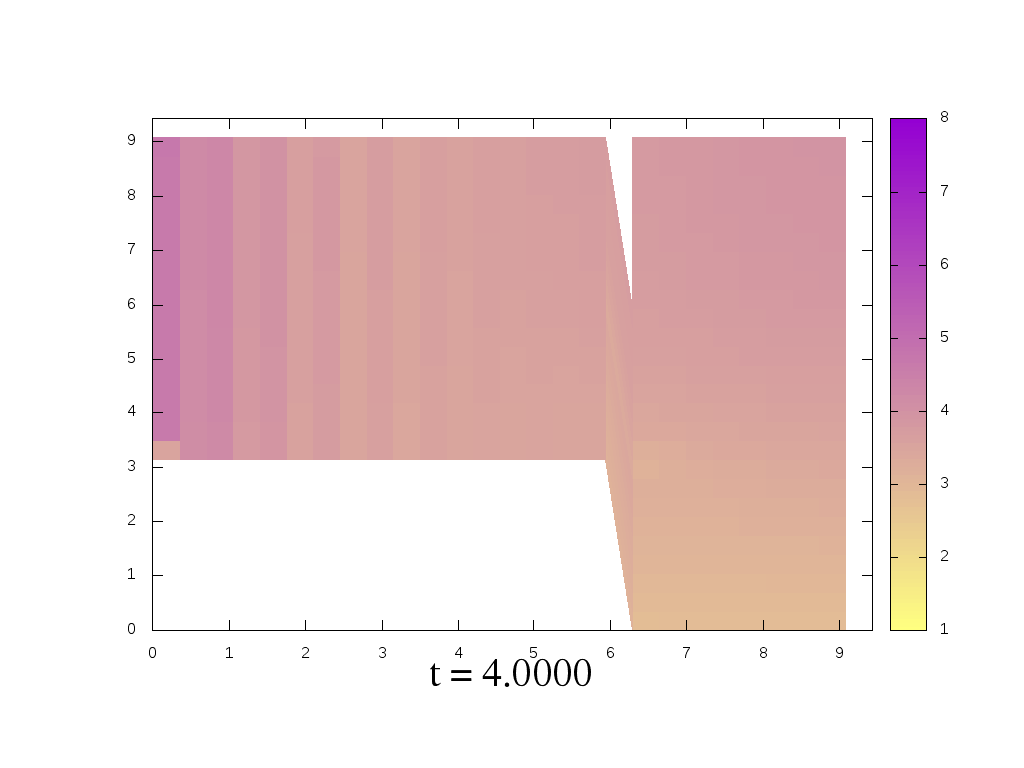
\includegraphics[width=1\linewidth]{./pics/0.1-10-10-21/g/8.png}}
\end{minipage}
\hfill
\begin{minipage}[h]{0.43\linewidth}
\center{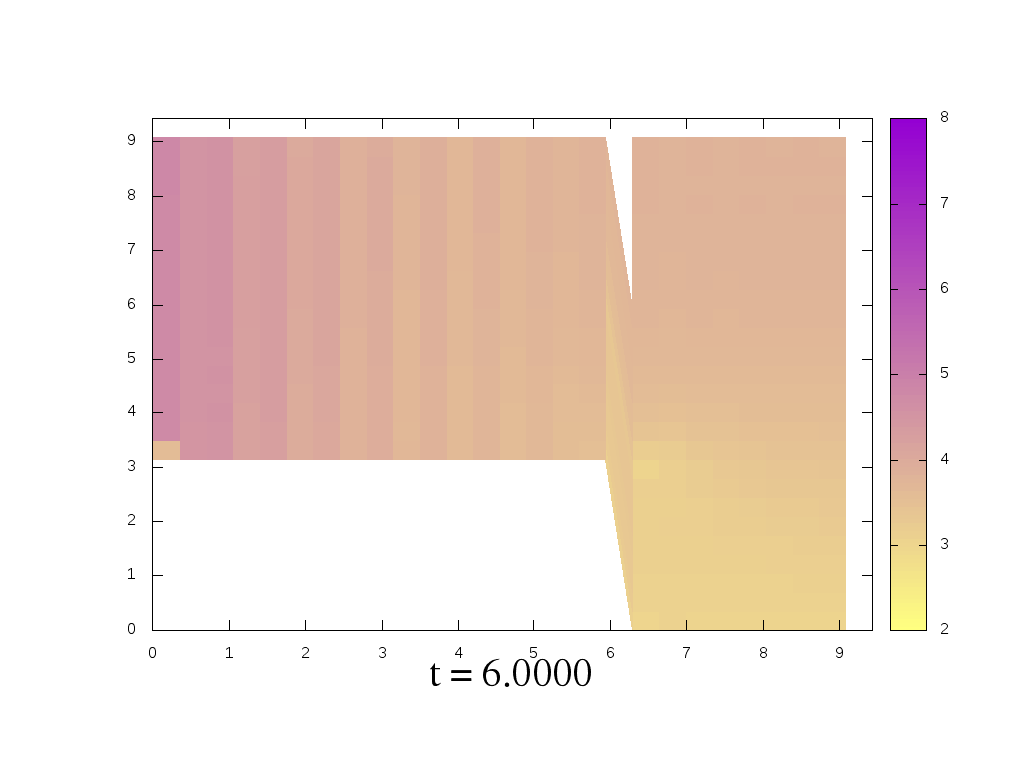
\includegraphics[width=1\linewidth]{./pics/0.1-10-10-21/g/12.png}}
\end{minipage}
\end{figure}

\begin{figure}[H]
\begin{minipage}[h]{0.43\linewidth}
\center{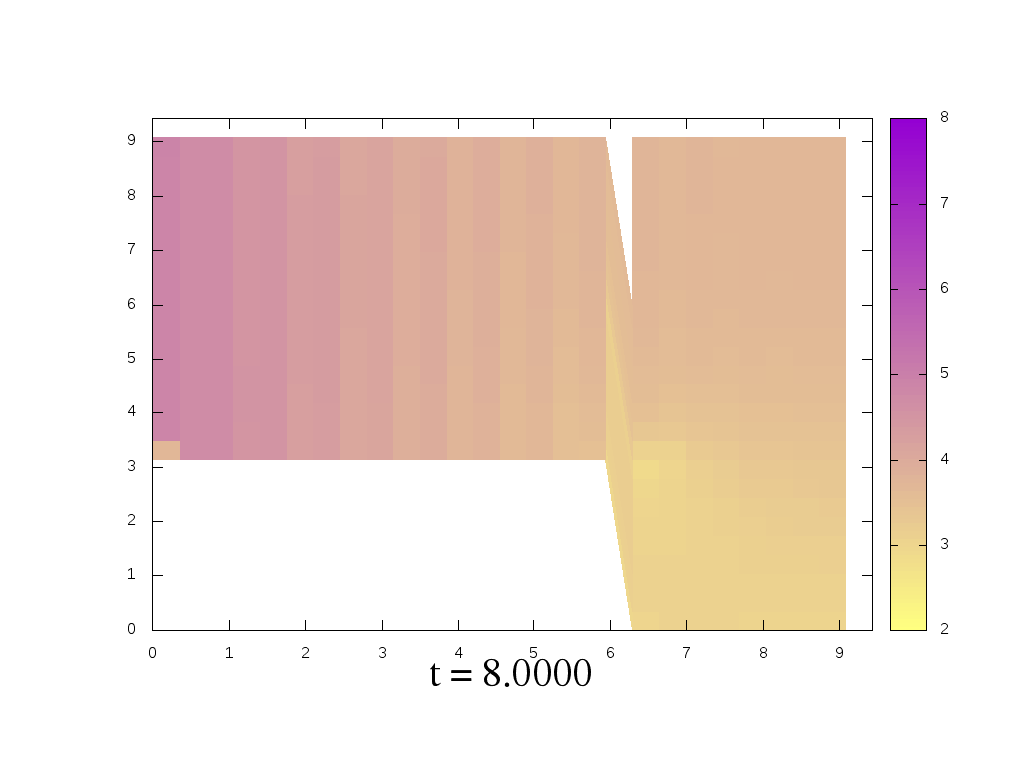
\includegraphics[width=1\linewidth]{./pics/0.1-10-10-21/g/16.png}}
\end{minipage}
\hfill
\begin{minipage}[h]{0.43\linewidth}
\center{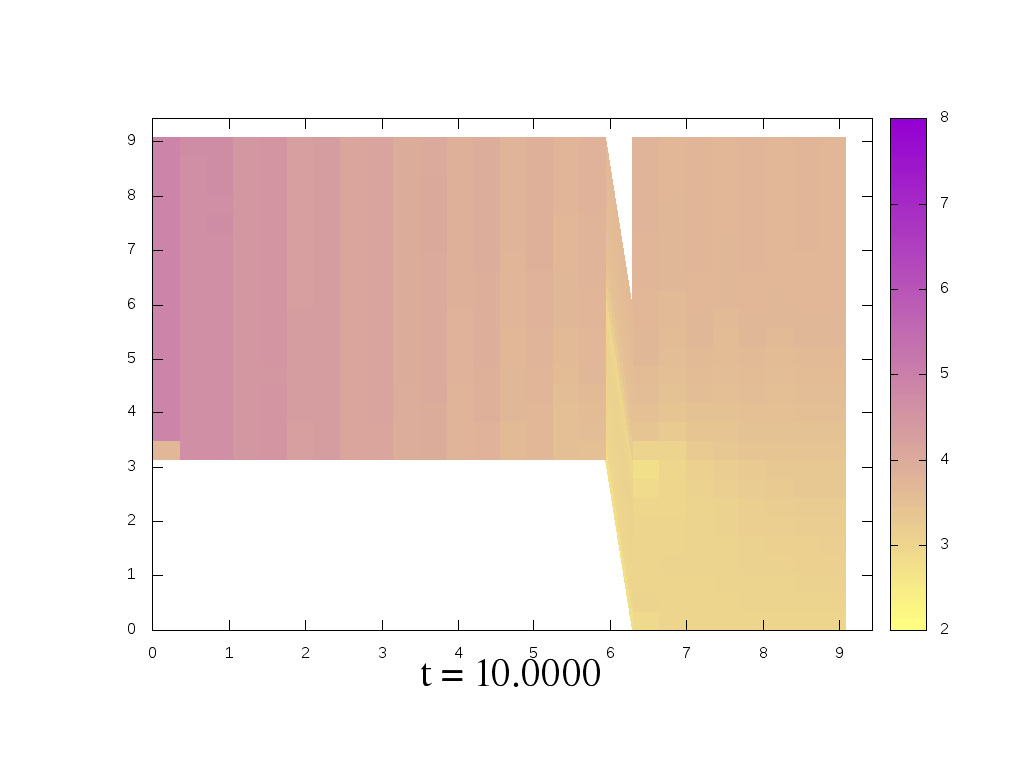
\includegraphics[width=1\linewidth]{./pics/0.1-10-10-21/g/20.png}}
\end{minipage}
\end{figure}


\subsubsection{$M_x=20$; $M_y=20$; $T=10$}
\begin{figure}[H]
\begin{minipage}[h]{0.43\linewidth}
\center{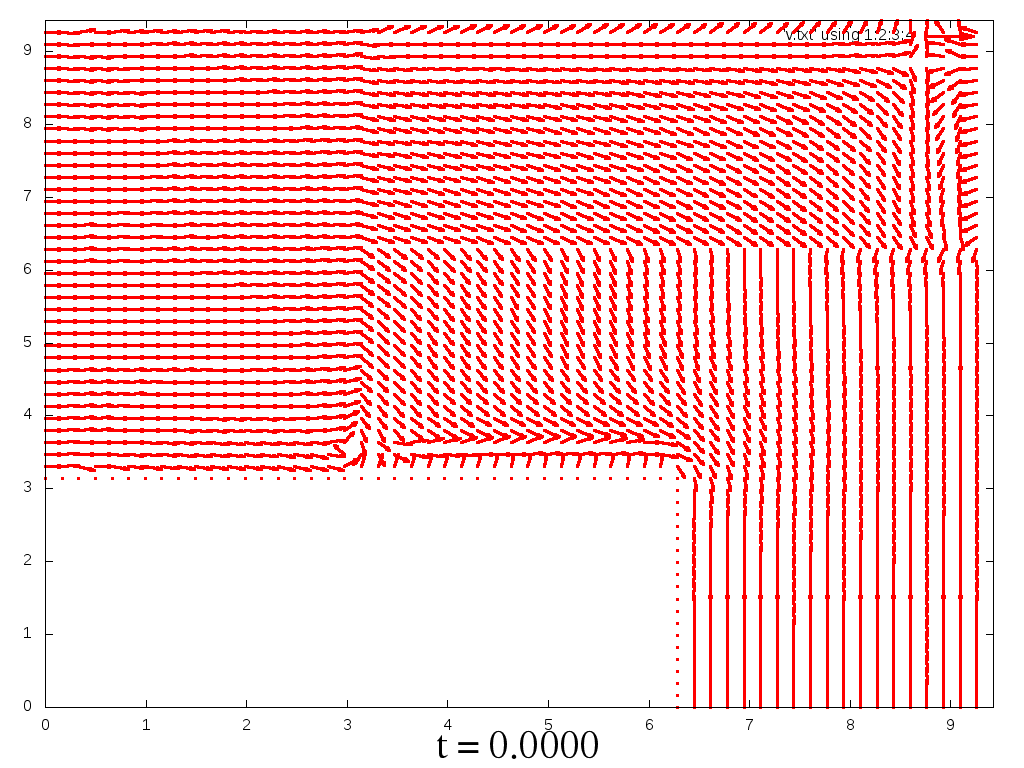
\includegraphics[width=1\linewidth]{./pics/0.1-20-10-21/v/0.png}}
\end{minipage}
\hfill
\begin{minipage}[h]{0.43\linewidth}
\center{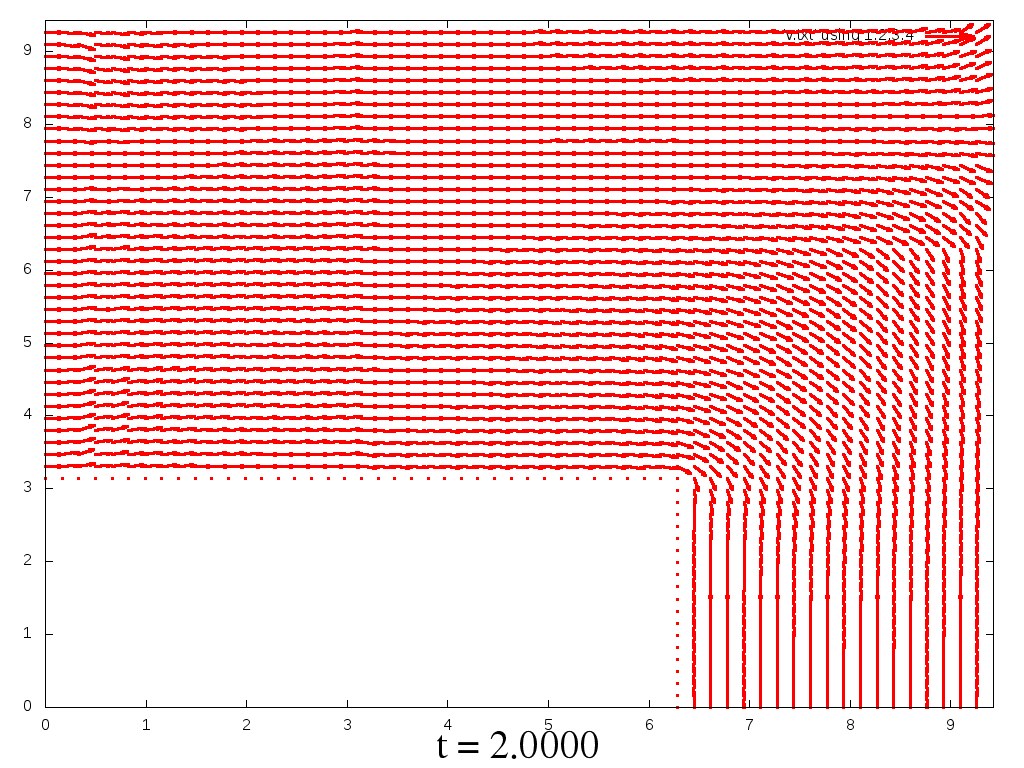
\includegraphics[width=1\linewidth]{./pics/0.1-20-10-21/v/4.png}}
\end{minipage}
\end{figure}

\begin{figure}[H]
\begin{minipage}[h]{0.43\linewidth}
\center{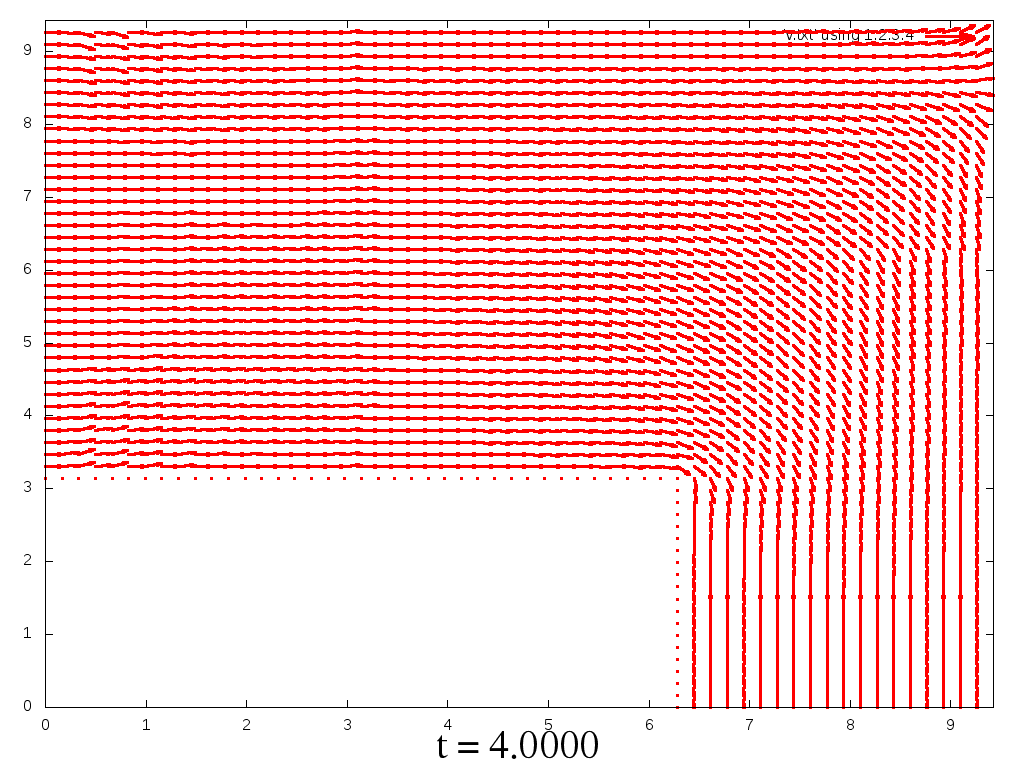
\includegraphics[width=1\linewidth]{./pics/0.1-20-10-21/v/8.png}}
\end{minipage}
\hfill
\begin{minipage}[h]{0.43\linewidth}
\center{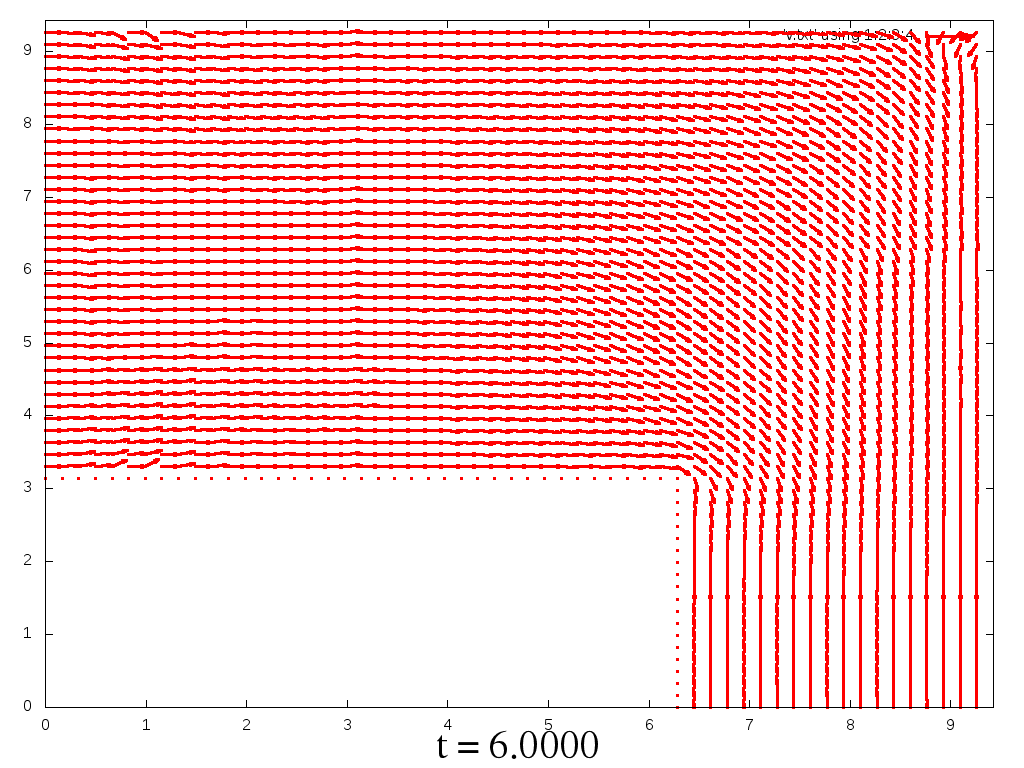
\includegraphics[width=1\linewidth]{./pics/0.1-20-10-21/v/12.png}}
\end{minipage}
\end{figure}

\begin{figure}[H]
\begin{minipage}[h]{0.43\linewidth}
\center{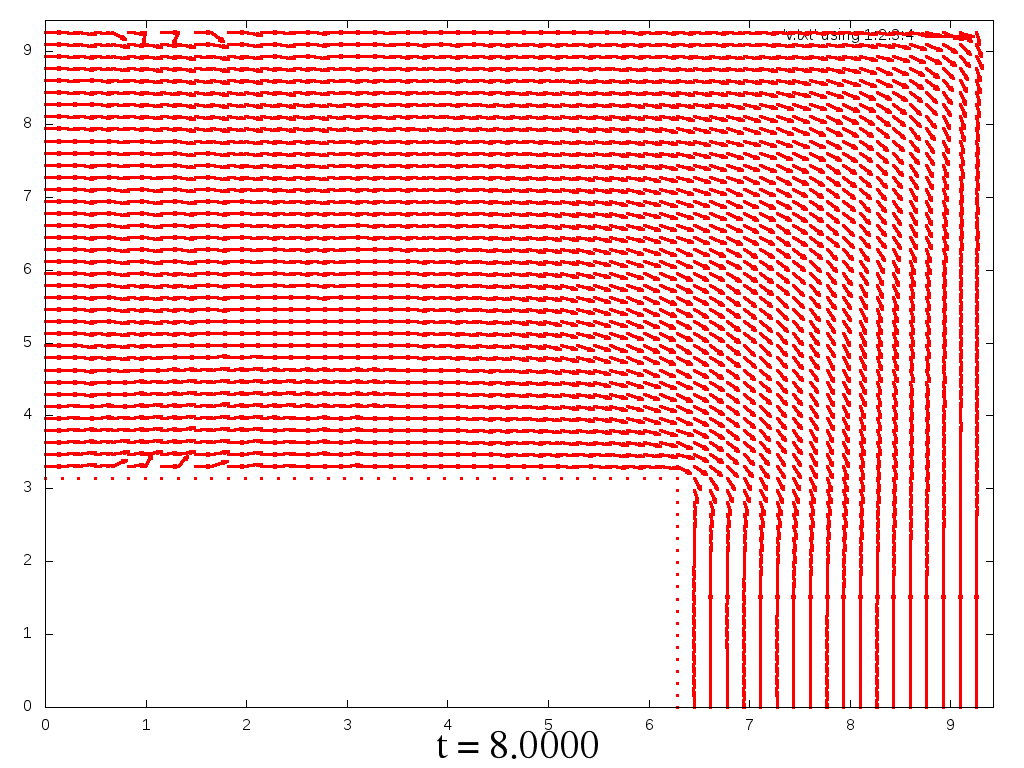
\includegraphics[width=1\linewidth]{./pics/0.1-20-10-21/v/16.png}}
\end{minipage}
\hfill
\begin{minipage}[h]{0.43\linewidth}
\center{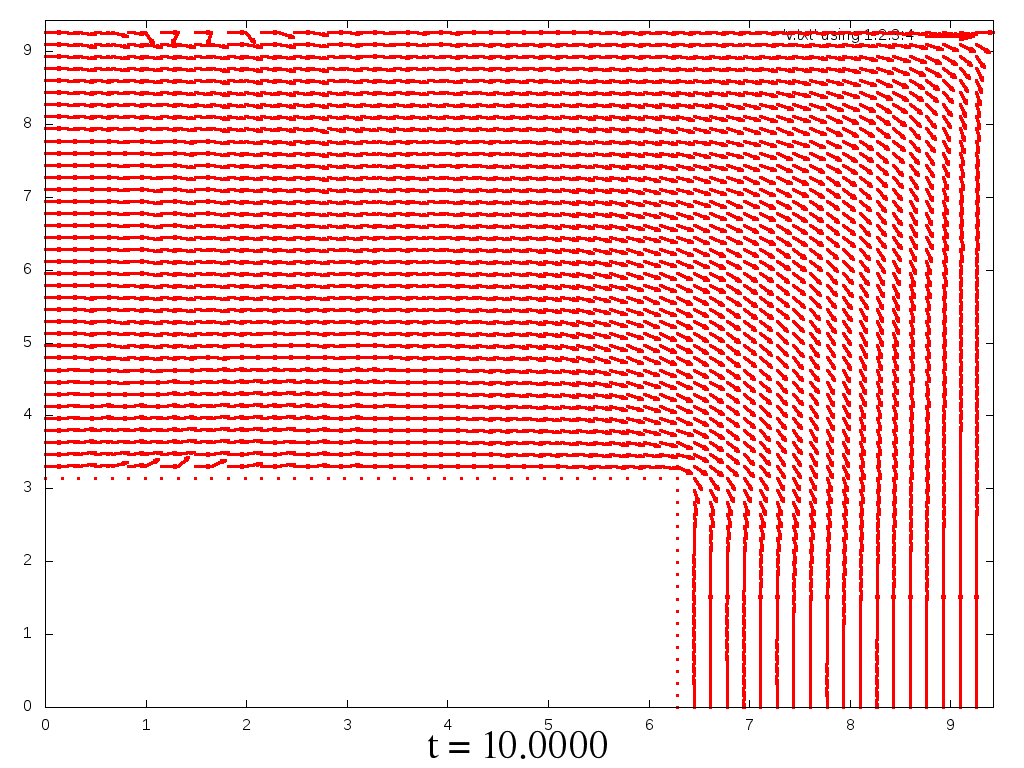
\includegraphics[width=1\linewidth]{./pics/0.1-20-10-21/v/20.png}}
\end{minipage}
\end{figure}

\begin{figure}[H]
\begin{minipage}[h]{0.43\linewidth}
\center{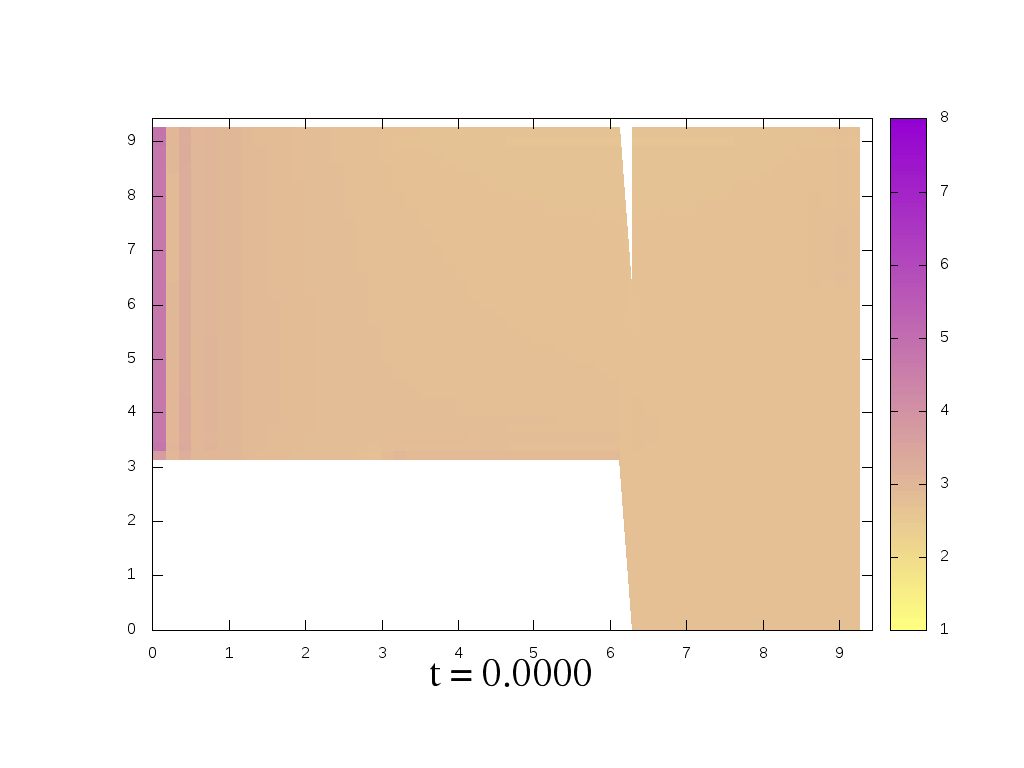
\includegraphics[width=1\linewidth]{./pics/0.1-20-10-21/g/0.png}}
\end{minipage}
\hfill
\begin{minipage}[h]{0.43\linewidth}
\center{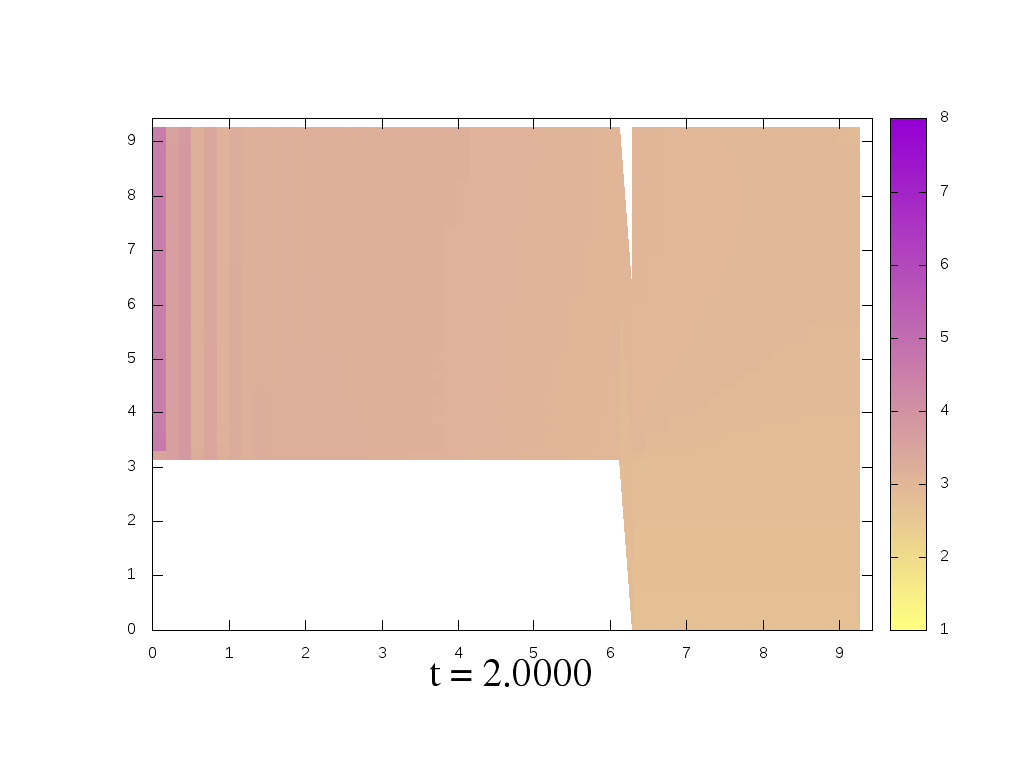
\includegraphics[width=1\linewidth]{./pics/0.1-20-10-21/g/4.png}}
\end{minipage}
\end{figure}

\begin{figure}[H]
\begin{minipage}[h]{0.43\linewidth}
\center{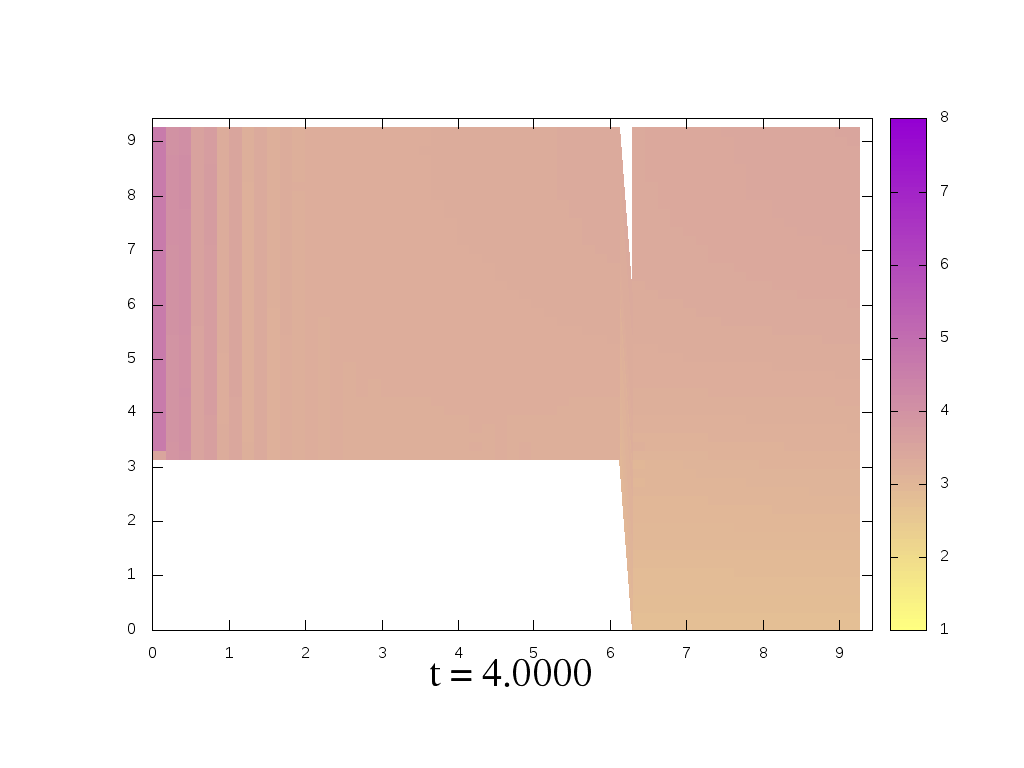
\includegraphics[width=1\linewidth]{./pics/0.1-20-10-21/g/8.png}}
\end{minipage}
\hfill
\begin{minipage}[h]{0.43\linewidth}
\center{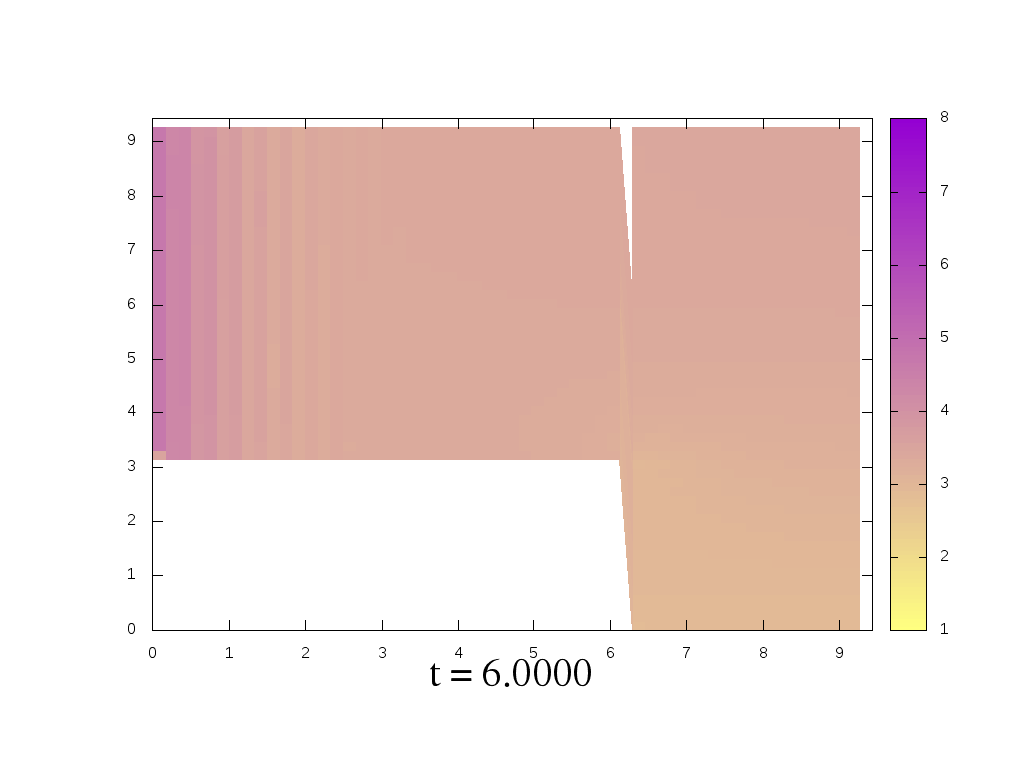
\includegraphics[width=1\linewidth]{./pics/0.1-20-10-21/g/12.png}}
\end{minipage}
\end{figure}

\begin{figure}[H]
\begin{minipage}[h]{0.43\linewidth}
\center{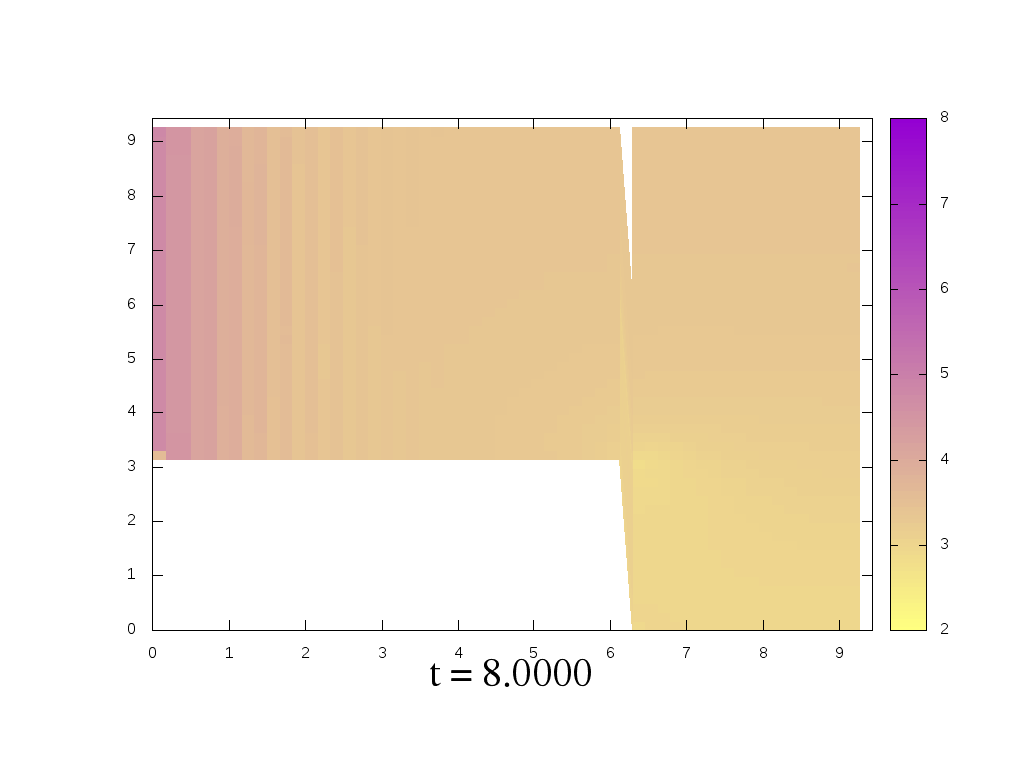
\includegraphics[width=1\linewidth]{./pics/0.1-20-10-21/g/16.png}}
\end{minipage}
\hfill
\begin{minipage}[h]{0.43\linewidth}
\center{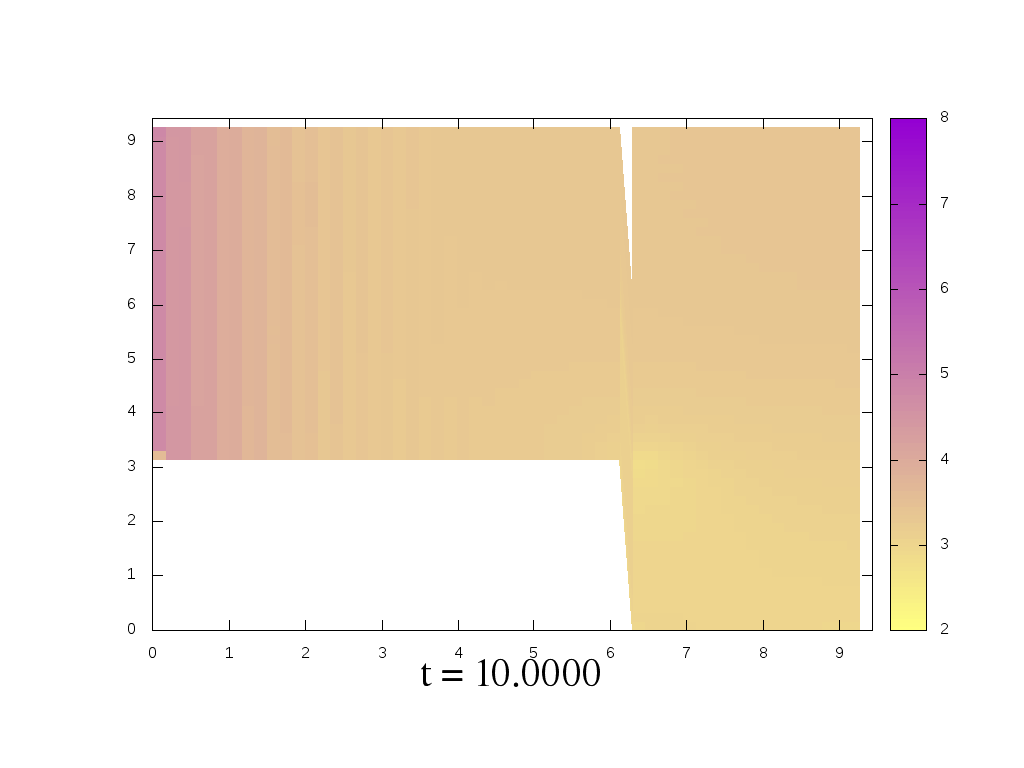
\includegraphics[width=1\linewidth]{./pics/0.1-20-10-21/g/20.png}}
\end{minipage}
\end{figure}



\subsubsection{$M_x=30$; $M_y=30$; $T=10$}
\begin{figure}[H]
\begin{minipage}[h]{0.43\linewidth}
\center{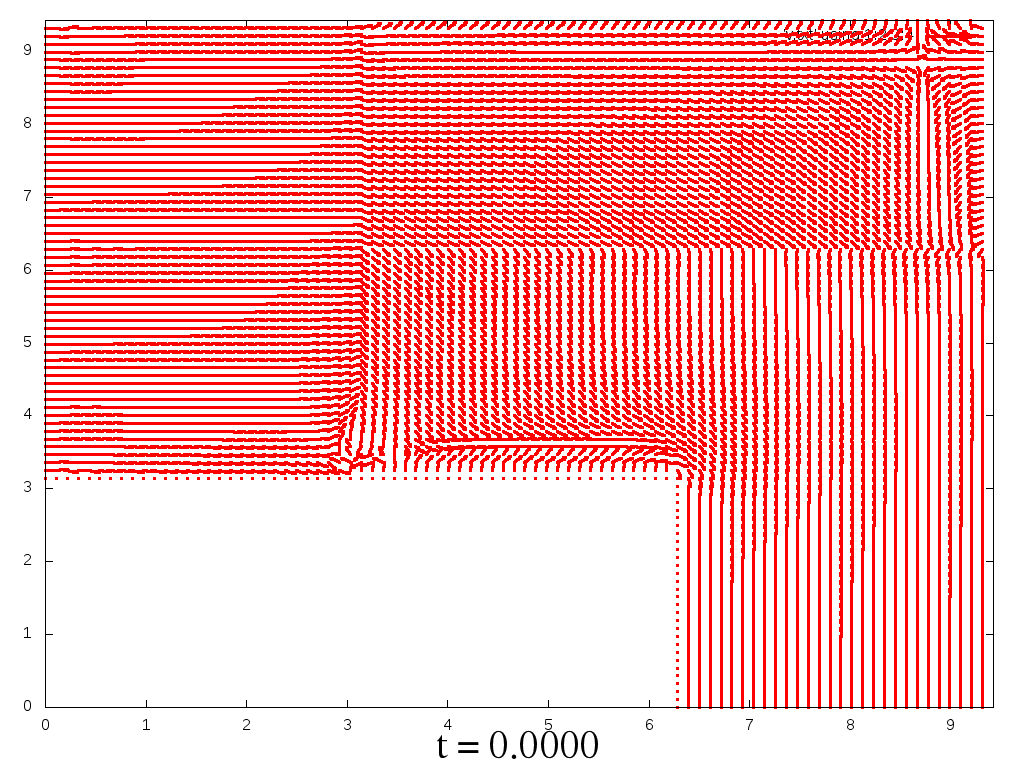
\includegraphics[width=1\linewidth]{./pics/0.1-30-10-21/v/0.png}}
\end{minipage}
\hfill
\begin{minipage}[h]{0.43\linewidth}
\center{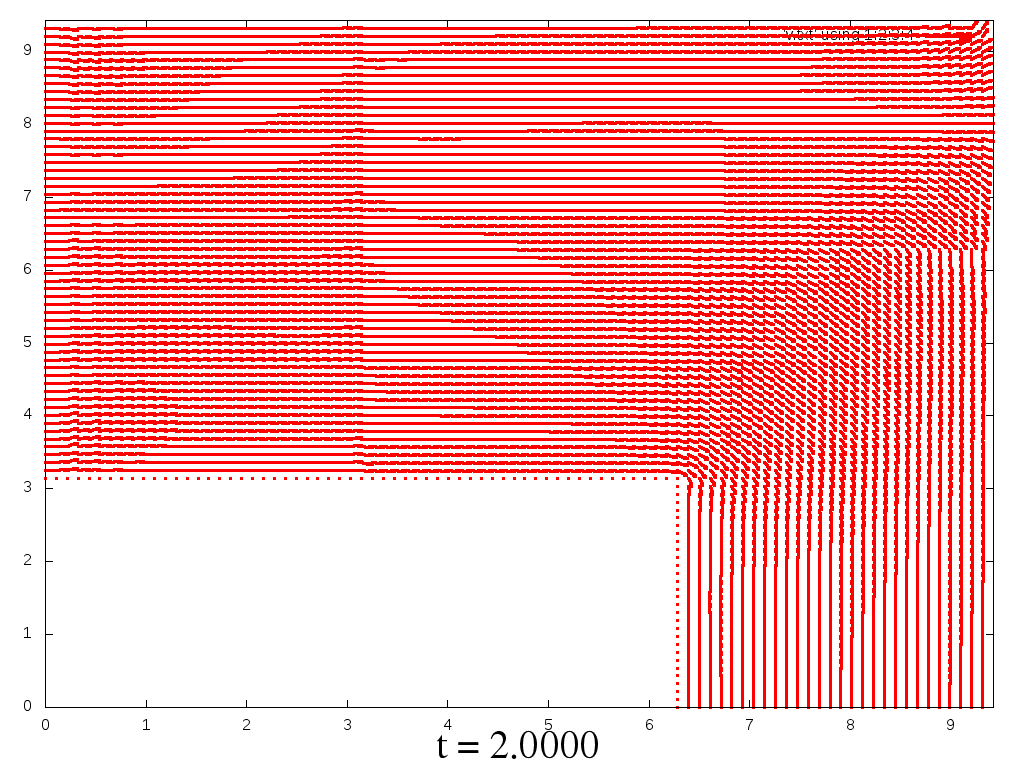
\includegraphics[width=1\linewidth]{./pics/0.1-30-10-21/v/4.png}}
\end{minipage}
\end{figure}

\begin{figure}[H]
\begin{minipage}[h]{0.43\linewidth}
\center{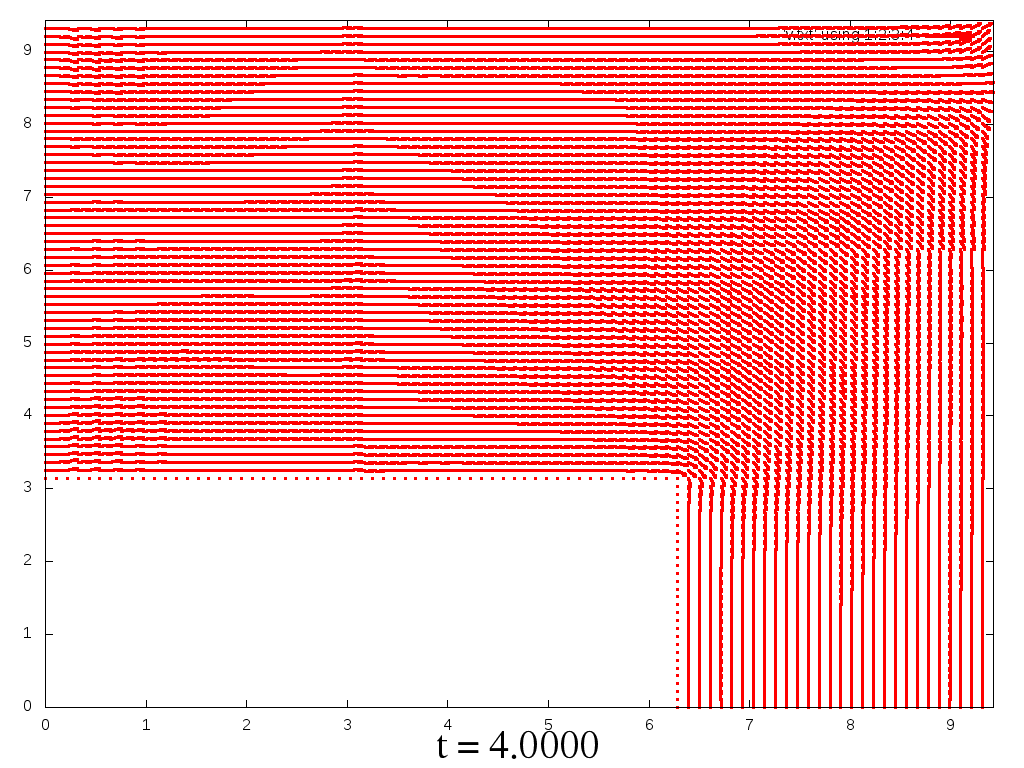
\includegraphics[width=1\linewidth]{./pics/0.1-30-10-21/v/8.png}}
\end{minipage}
\hfill
\begin{minipage}[h]{0.43\linewidth}
\center{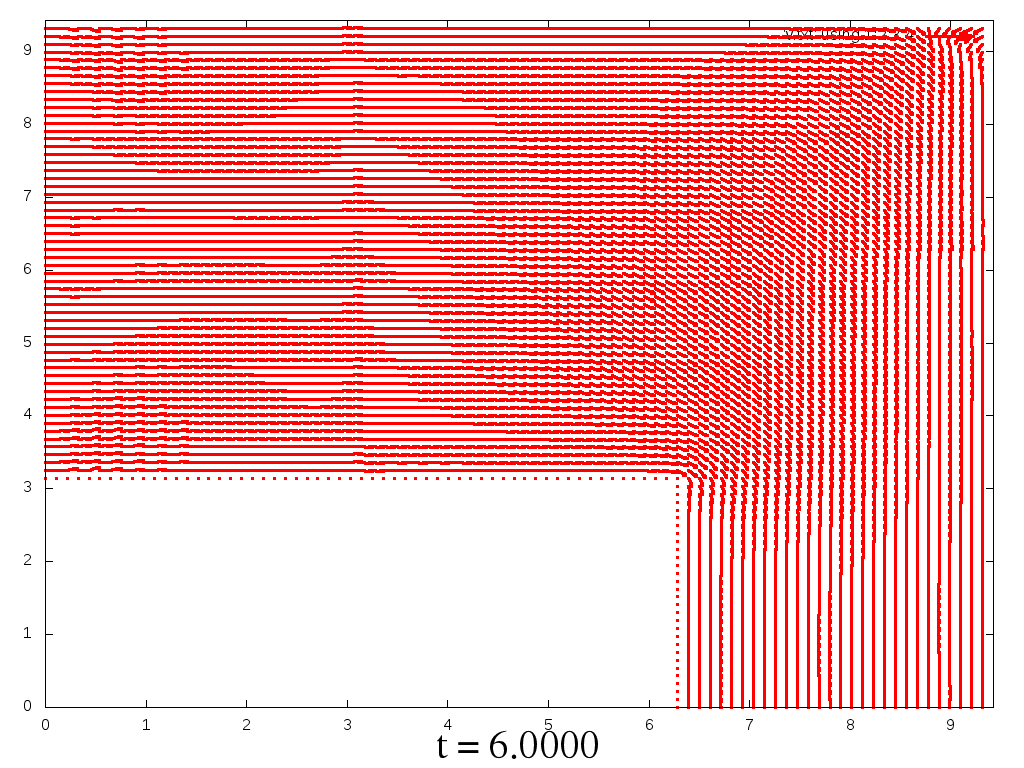
\includegraphics[width=1\linewidth]{./pics/0.1-30-10-21/v/12.png}}
\end{minipage}
\end{figure}

\begin{figure}[H]
\begin{minipage}[h]{0.43\linewidth}
\center{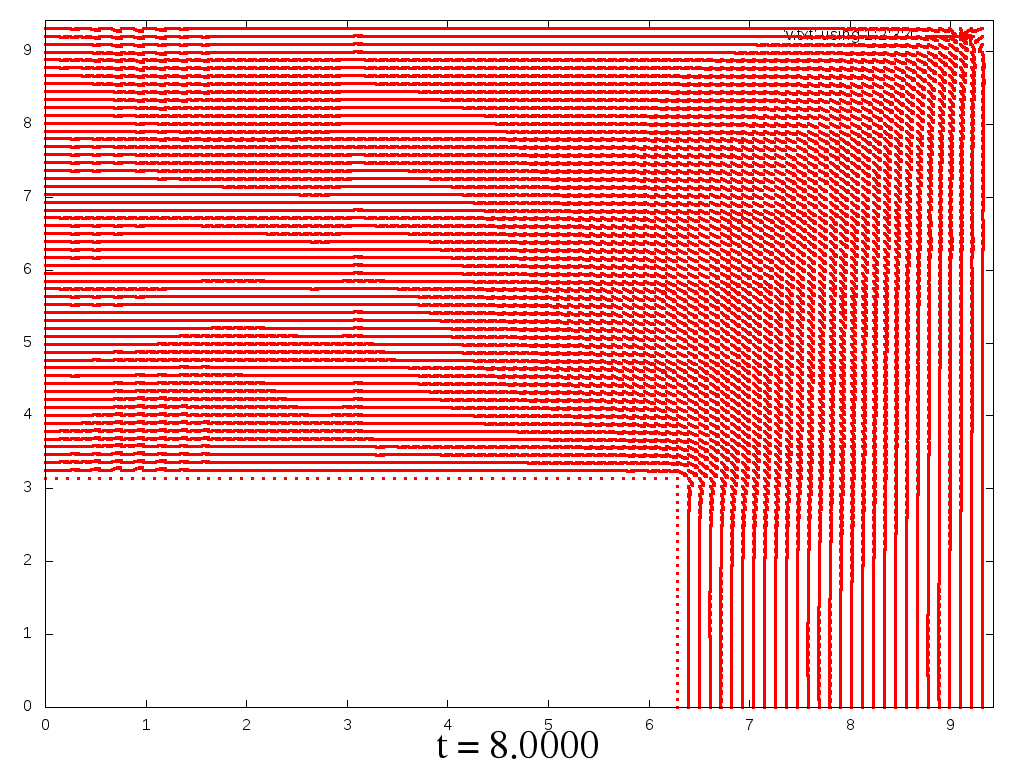
\includegraphics[width=1\linewidth]{./pics/0.1-30-10-21/v/16.png}}
\end{minipage}
\hfill
\begin{minipage}[h]{0.43\linewidth}
\center{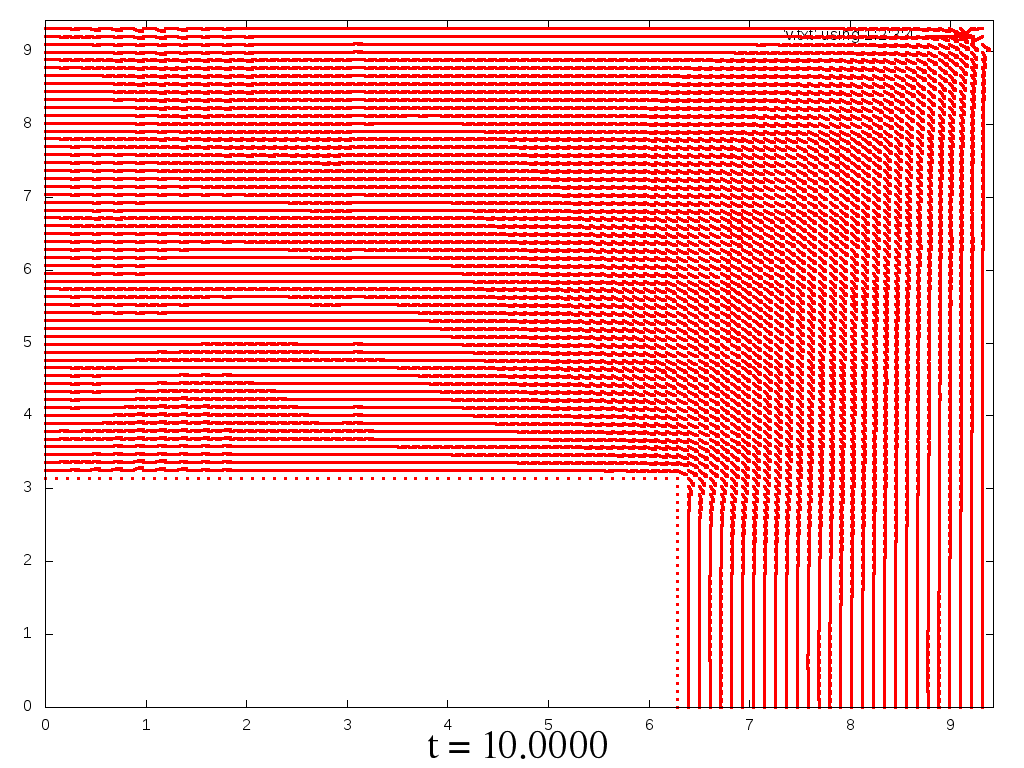
\includegraphics[width=1\linewidth]{./pics/0.1-30-10-21/v/20.png}}
\end{minipage}
\end{figure}

\begin{figure}[H]
\begin{minipage}[h]{0.43\linewidth}
\center{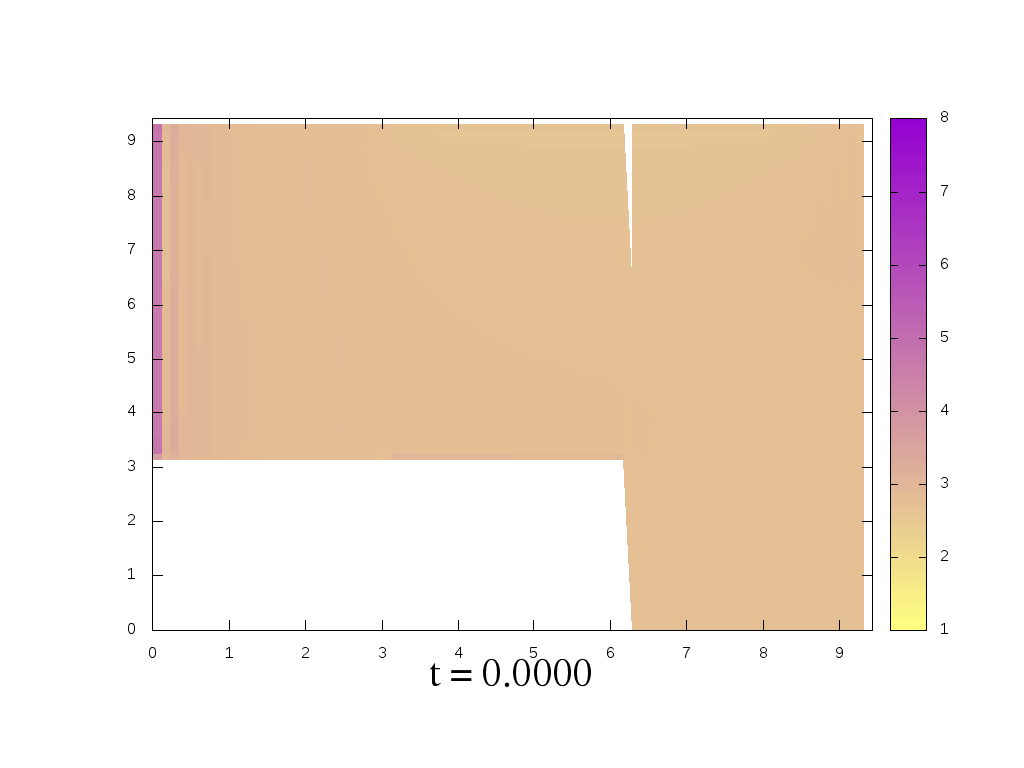
\includegraphics[width=1\linewidth]{./pics/0.1-30-10-21/g/0.png}}
\end{minipage}
\hfill
\begin{minipage}[h]{0.43\linewidth}
\center{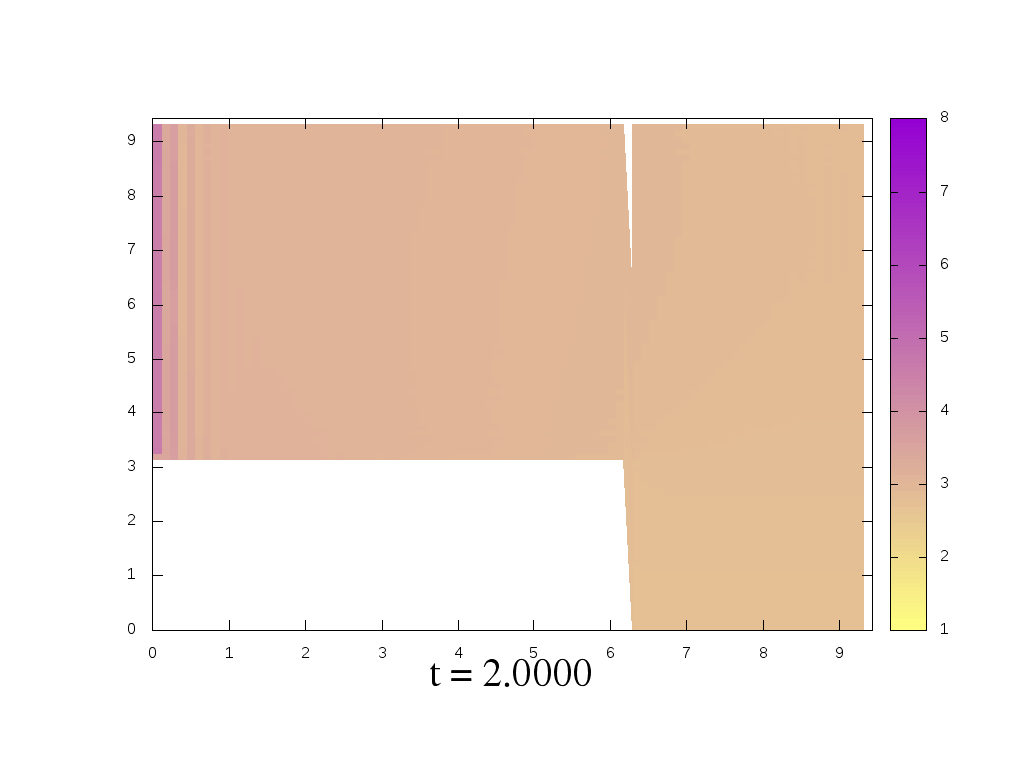
\includegraphics[width=1\linewidth]{./pics/0.1-30-10-21/g/4.png}}
\end{minipage}
\end{figure}

\begin{figure}[H]
\begin{minipage}[h]{0.43\linewidth}
\center{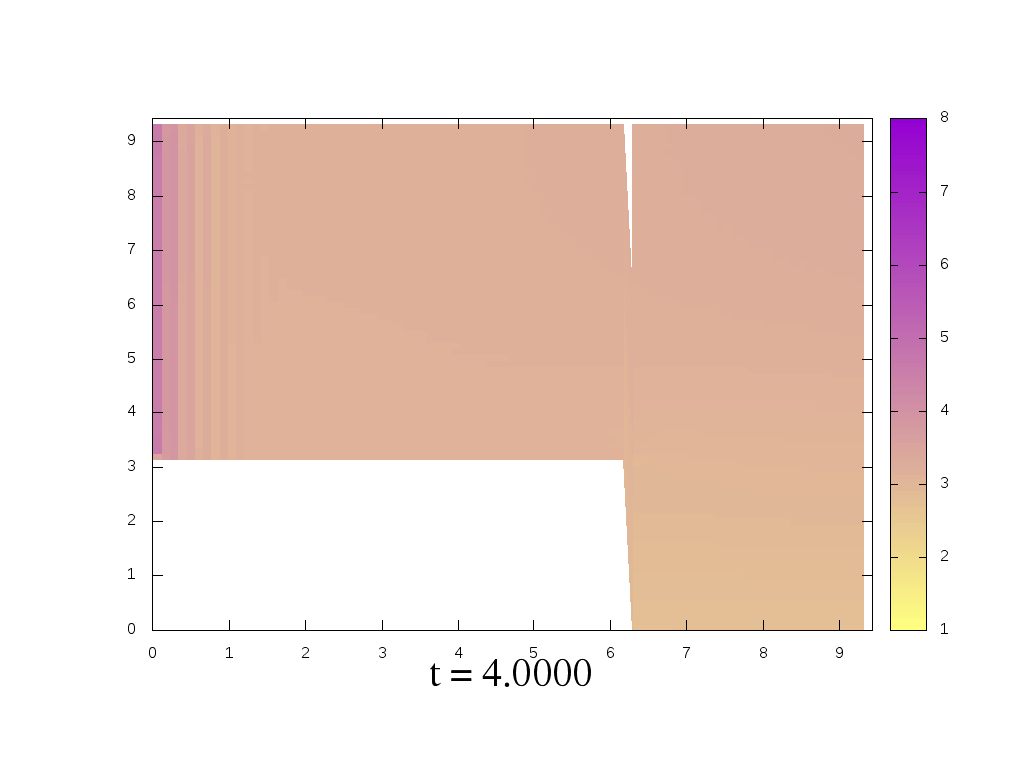
\includegraphics[width=1\linewidth]{./pics/0.1-30-10-21/g/8.png}}
\end{minipage}
\hfill
\begin{minipage}[h]{0.43\linewidth}
\center{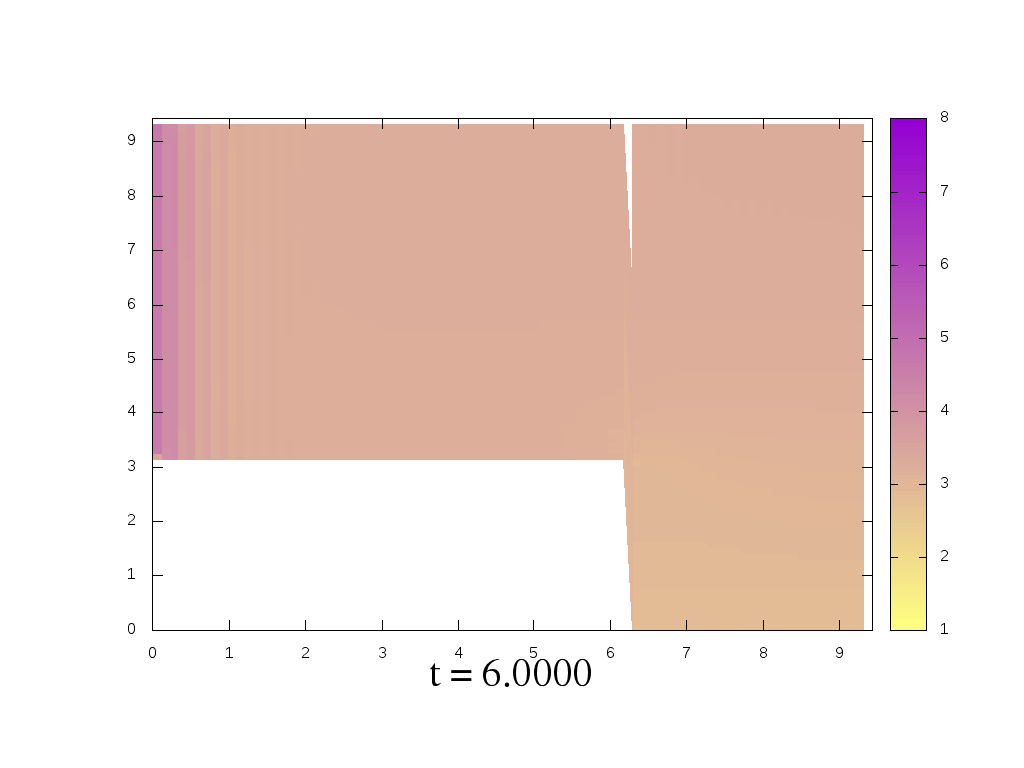
\includegraphics[width=1\linewidth]{./pics/0.1-30-10-21/g/12.png}}
\end{minipage}
\end{figure}

\begin{figure}[H]
\begin{minipage}[h]{0.43\linewidth}
\center{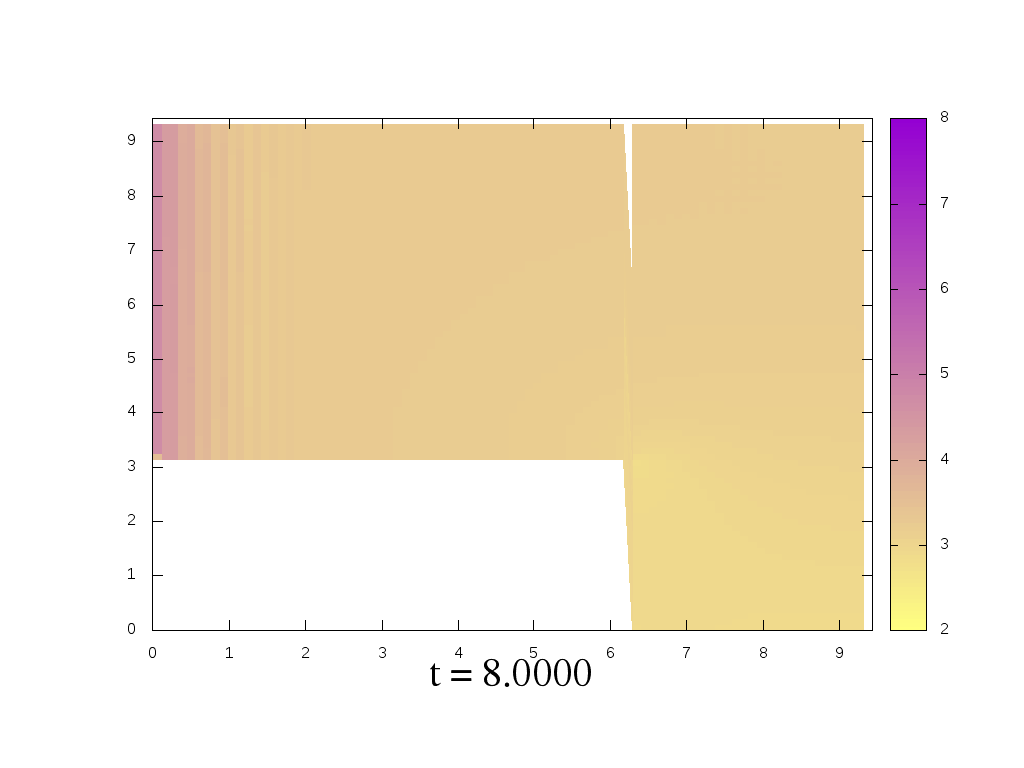
\includegraphics[width=1\linewidth]{./pics/0.1-30-10-21/g/16.png}}
\end{minipage}
\hfill
\begin{minipage}[h]{0.43\linewidth}
\center{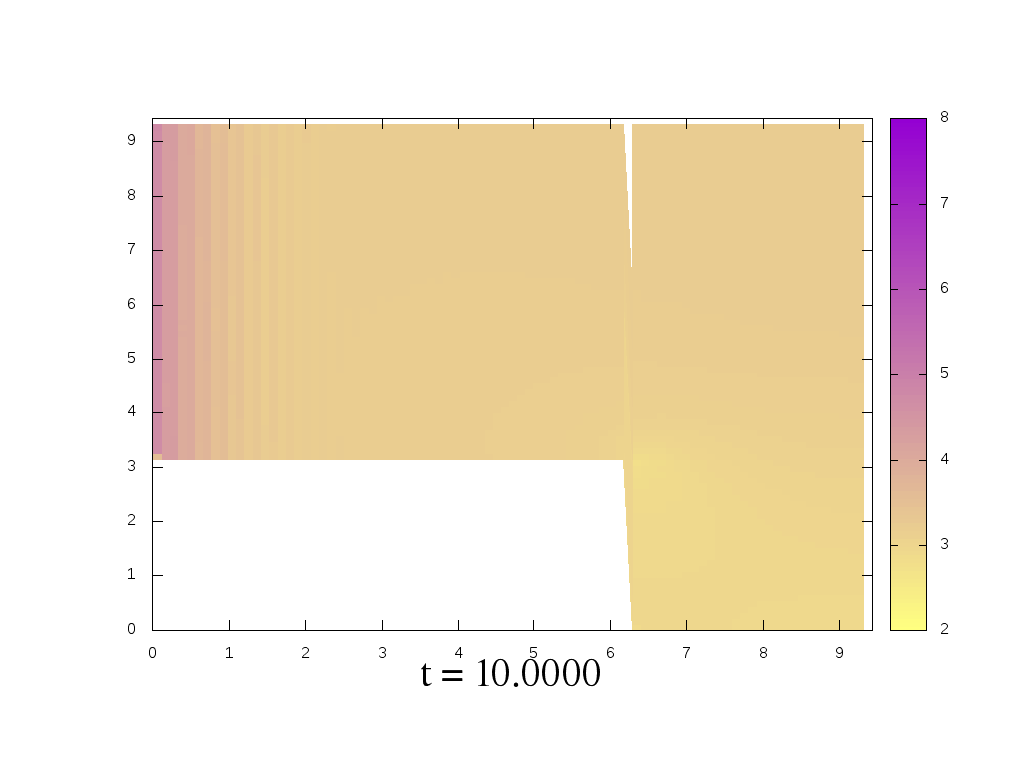
\includegraphics[width=1\linewidth]{./pics/0.1-30-10-21/g/20.png}}
\end{minipage}
\end{figure}



\subsubsection{$M_x=10$; $M_y=10$; $T=50$}
\begin{figure}[H]
\begin{minipage}[h]{0.43\linewidth}
\center{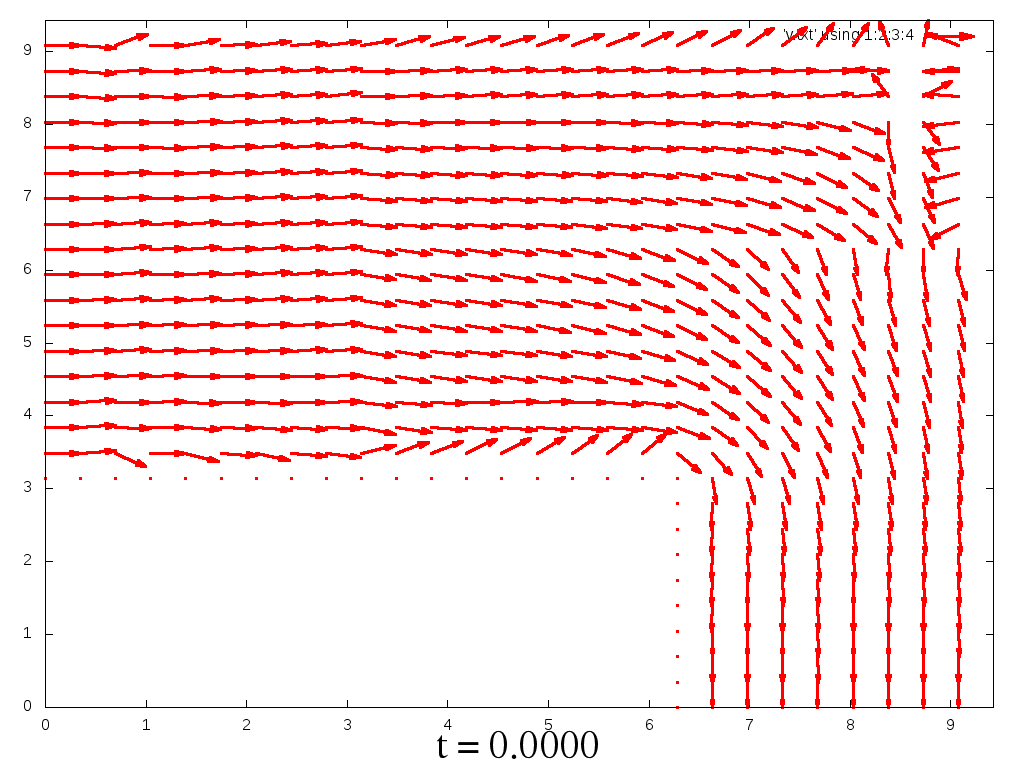
\includegraphics[width=1\linewidth]{./pics/0.1-10-50-51/v/0.png}}
\end{minipage}
\hfill
\begin{minipage}[h]{0.43\linewidth}
\center{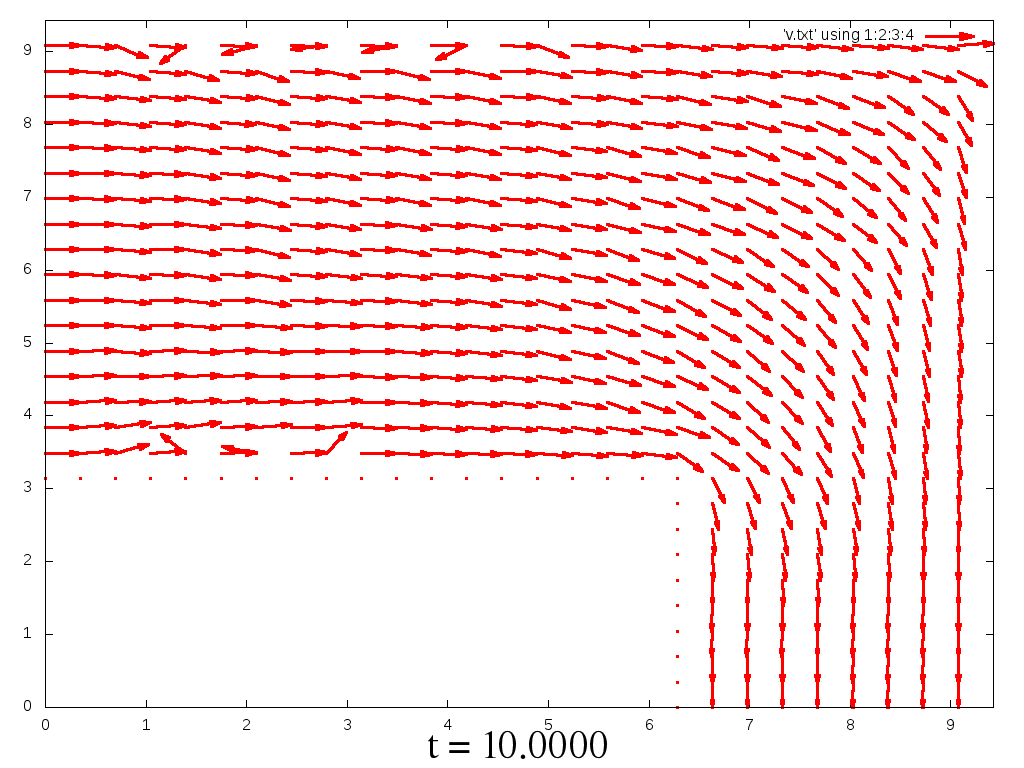
\includegraphics[width=1\linewidth]{./pics/0.1-10-50-51/v/10.png}}
\end{minipage}
\end{figure}

\begin{figure}[H]
\begin{minipage}[h]{0.43\linewidth}
\center{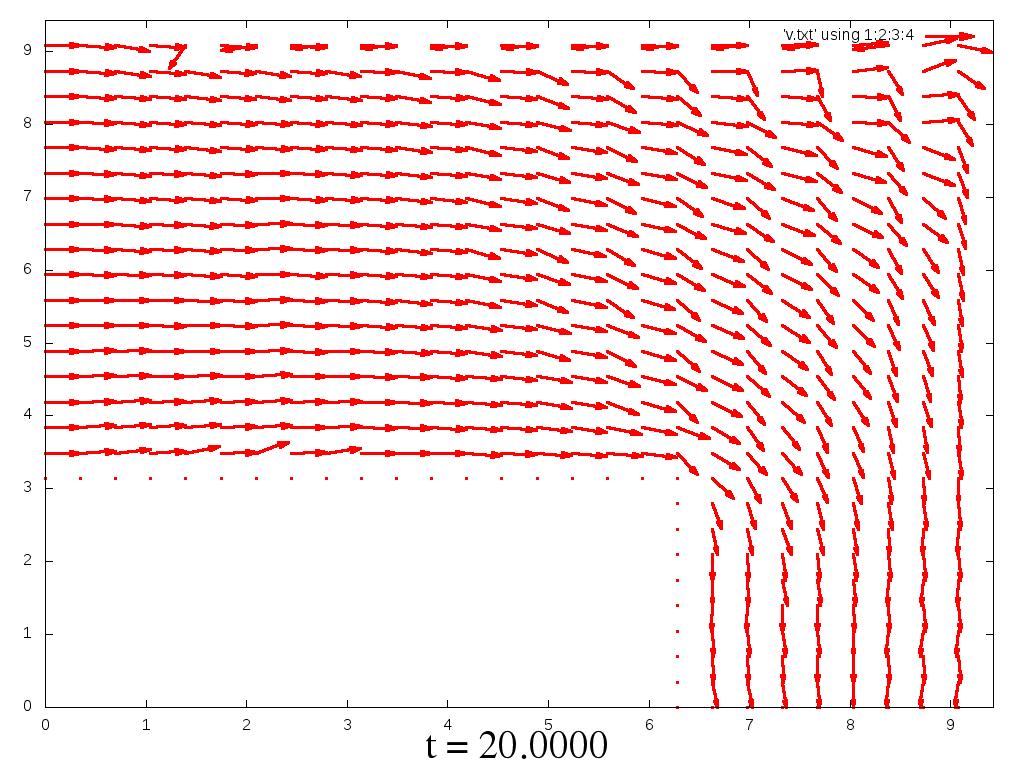
\includegraphics[width=1\linewidth]{./pics/0.1-10-50-51/v/20.png}}
\end{minipage}
\hfill
\begin{minipage}[h]{0.43\linewidth}
\center{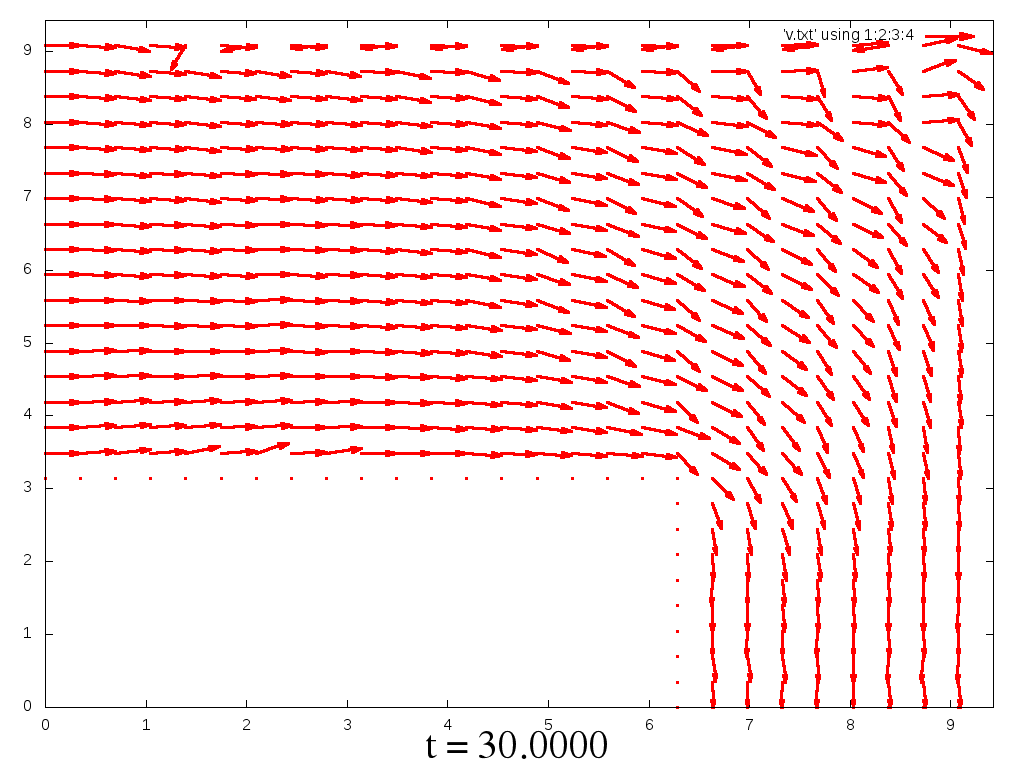
\includegraphics[width=1\linewidth]{./pics/0.1-10-50-51/v/30.png}}
\end{minipage}
\end{figure}

\begin{figure}[H]
\begin{minipage}[h]{0.43\linewidth}
\center{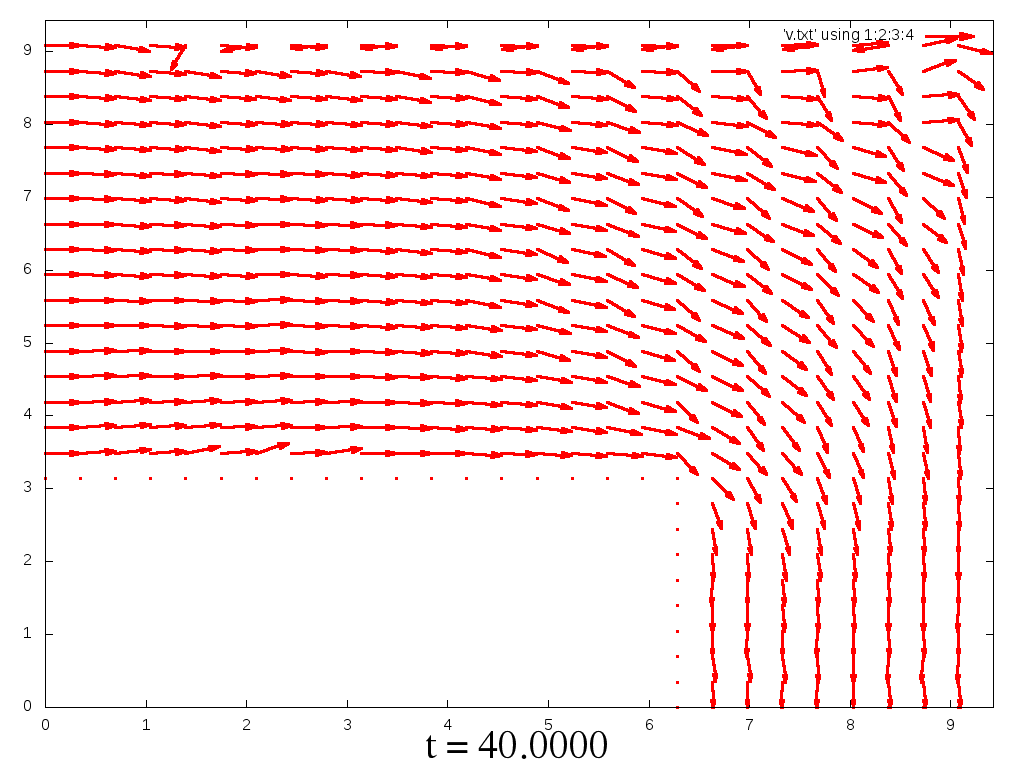
\includegraphics[width=1\linewidth]{./pics/0.1-10-50-51/v/40.png}}
\end{minipage}
\hfill
\begin{minipage}[h]{0.43\linewidth}
\center{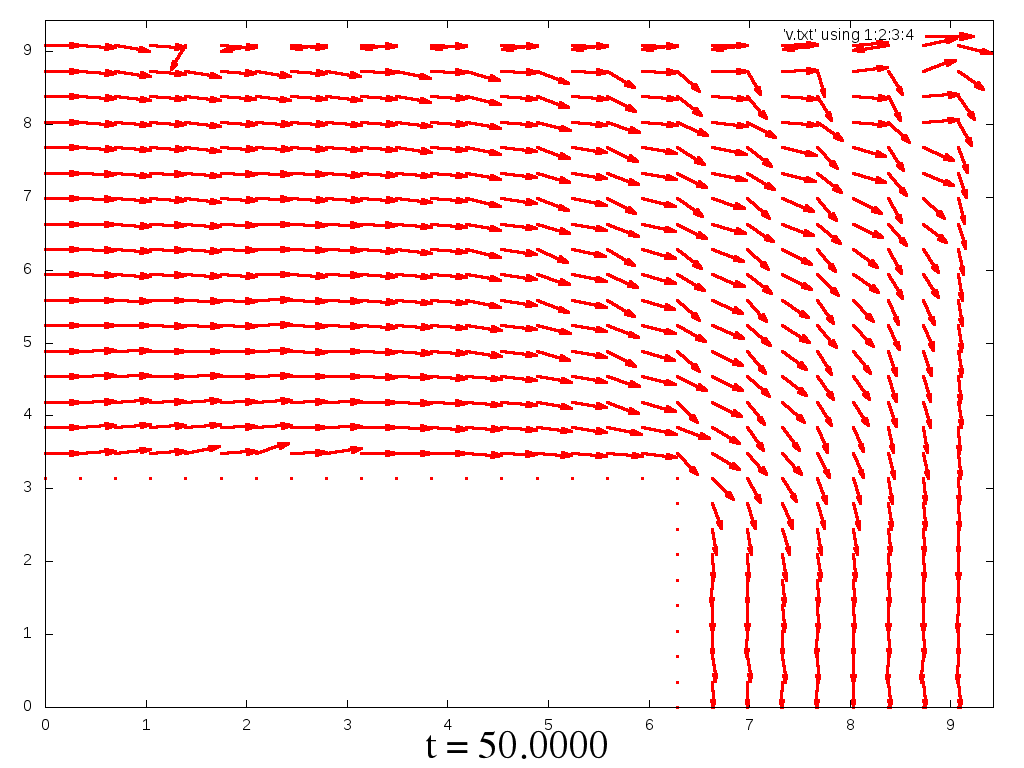
\includegraphics[width=1\linewidth]{./pics/0.1-10-50-51/v/50.png}}
\end{minipage}
\end{figure}

\begin{figure}[H]
\begin{minipage}[h]{0.43\linewidth}
\center{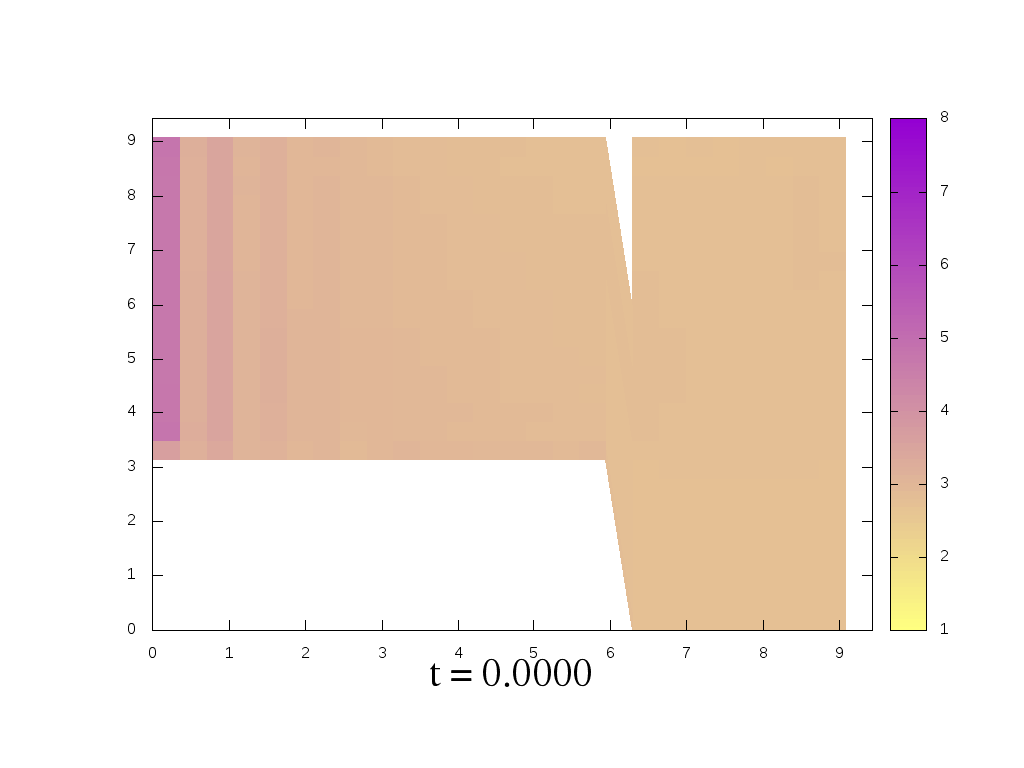
\includegraphics[width=1\linewidth]{./pics/0.1-10-50-51/g/0.png}}
\end{minipage}
\hfill
\begin{minipage}[h]{0.43\linewidth}
\center{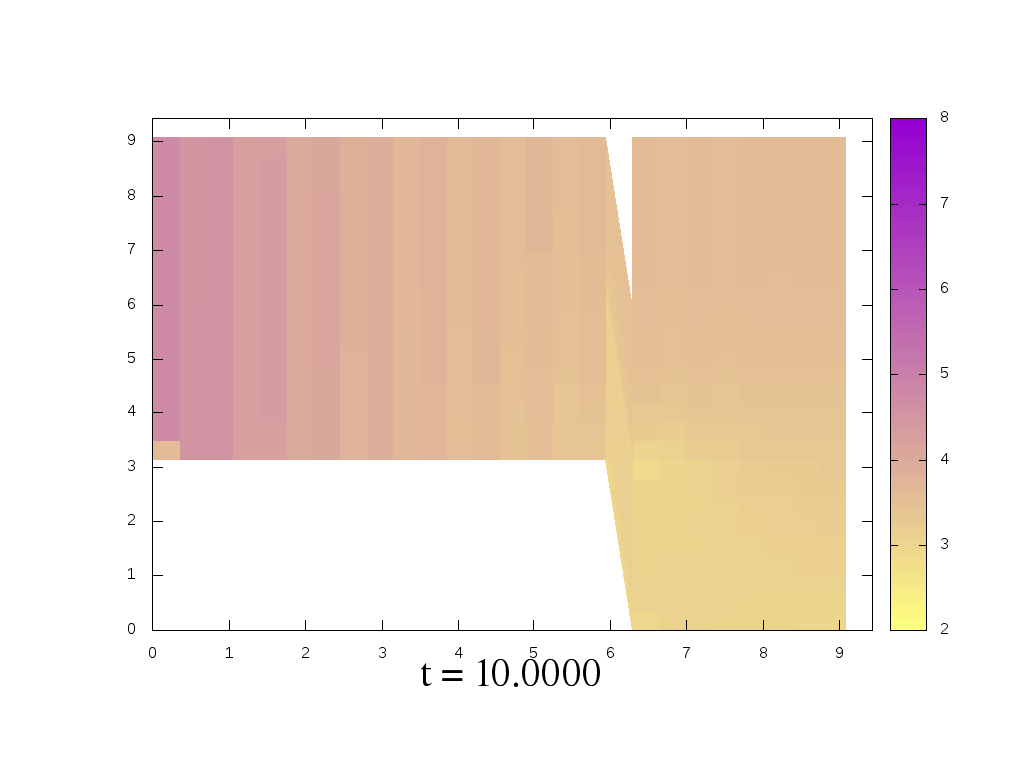
\includegraphics[width=1\linewidth]{./pics/0.1-10-50-51/g/10.png}}
\end{minipage}
\end{figure}

\begin{figure}[H]
\begin{minipage}[h]{0.43\linewidth}
\center{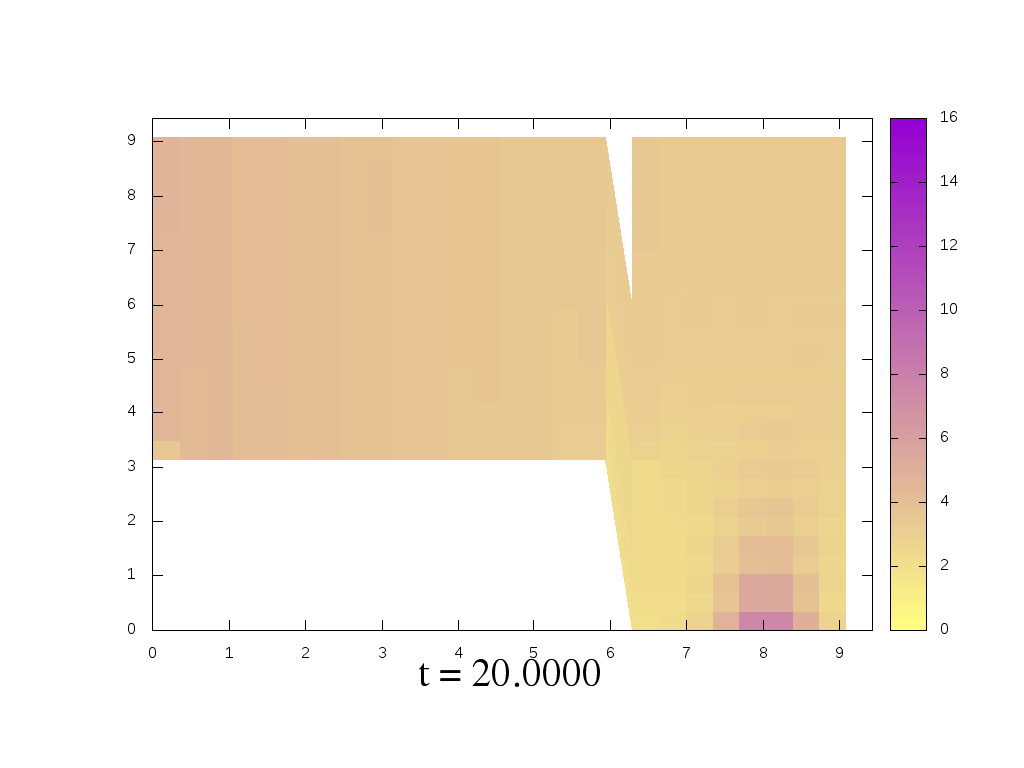
\includegraphics[width=1\linewidth]{./pics/0.1-10-50-51/g/20.png}}
\end{minipage}
\hfill
\begin{minipage}[h]{0.43\linewidth}
\center{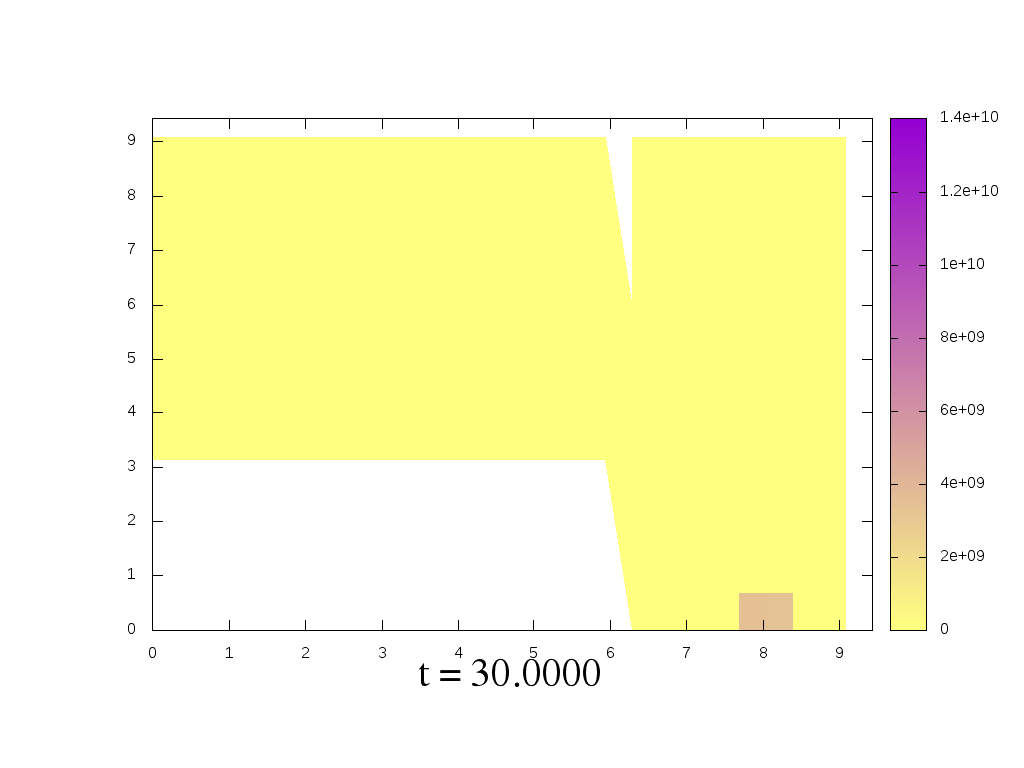
\includegraphics[width=1\linewidth]{./pics/0.1-10-50-51/g/30.png}}
\end{minipage}
\end{figure}

\begin{figure}[H]
\begin{minipage}[h]{0.43\linewidth}
\center{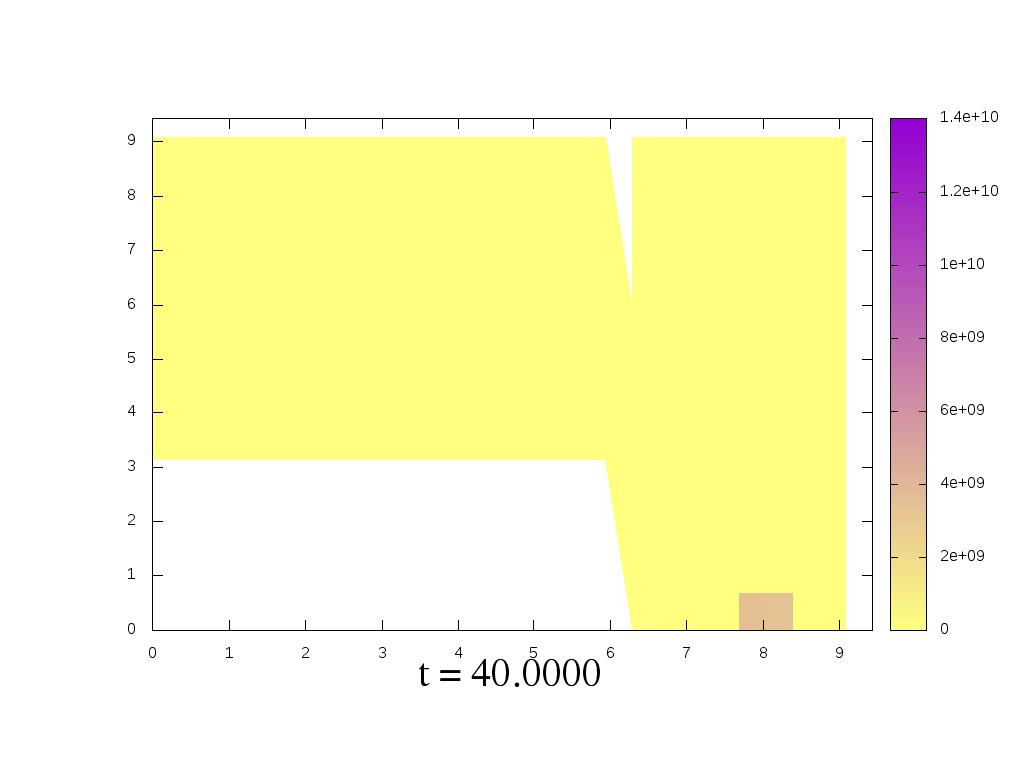
\includegraphics[width=1\linewidth]{./pics/0.1-10-50-51/g/40.png}}
\end{minipage}
\hfill
\begin{minipage}[h]{0.43\linewidth}
\center{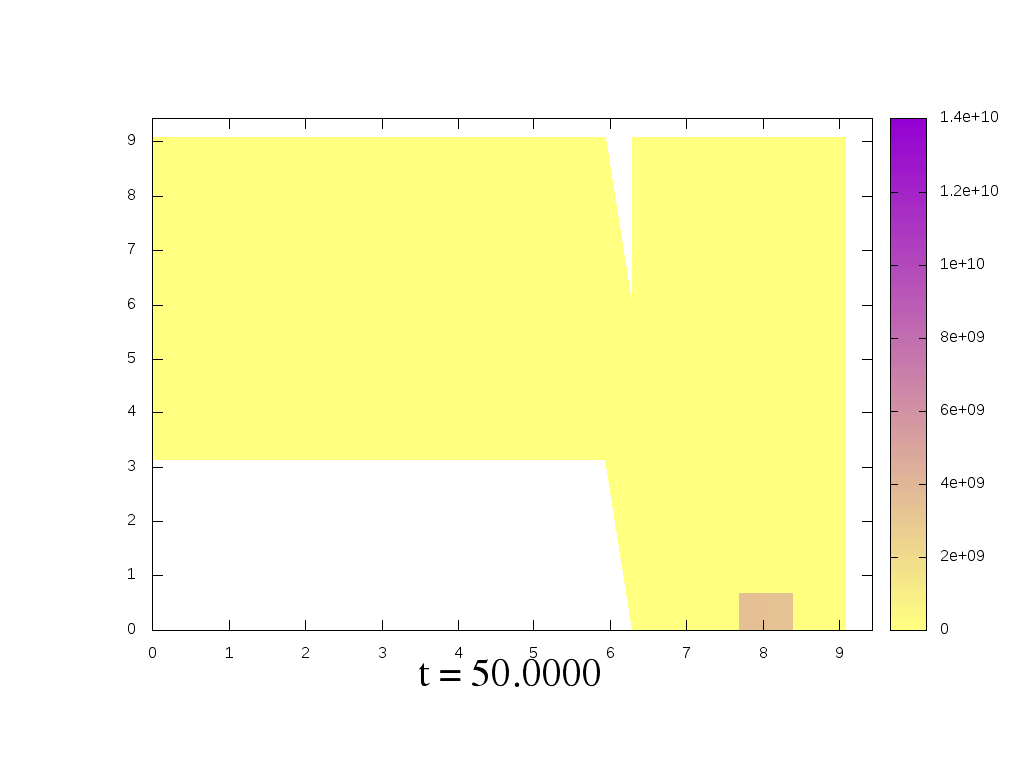
\includegraphics[width=1\linewidth]{./pics/0.1-10-50-51/g/50.png}}
\end{minipage}
\end{figure}




\subsubsection{$M_x=30$; $M_y=30$; $T=50$}
\begin{figure}[H]
\begin{minipage}[h]{0.43\linewidth}
\center{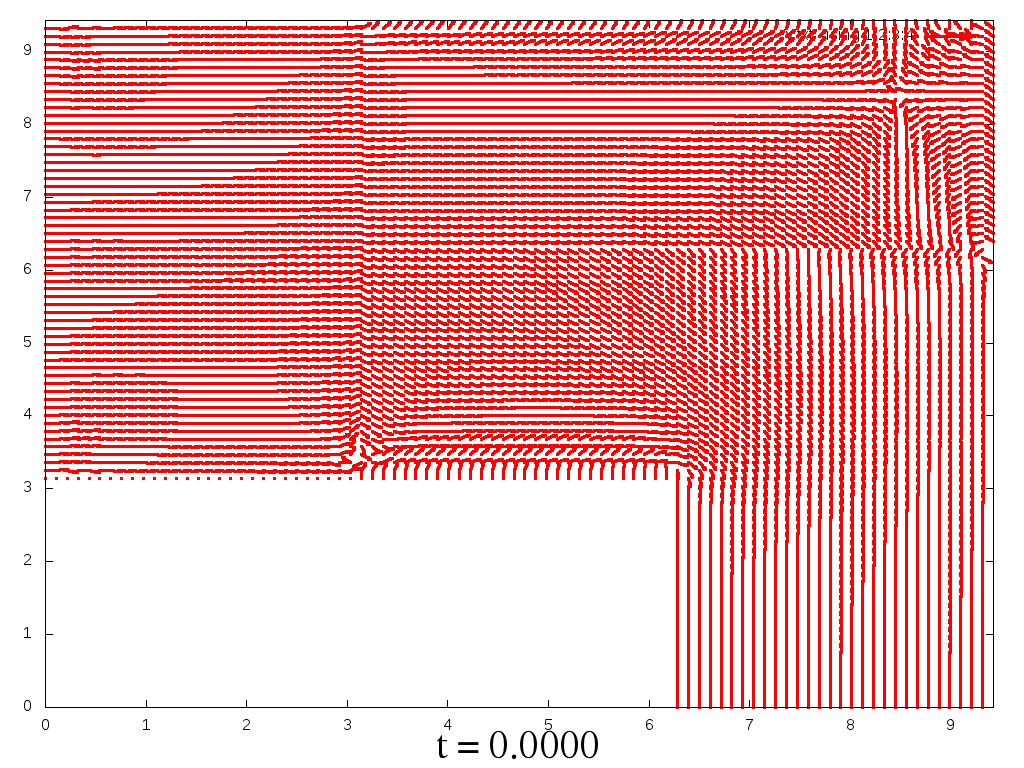
\includegraphics[width=1\linewidth]{./pics/0.1-30-50-51/v/0.png}}
\end{minipage}
\hfill
\begin{minipage}[h]{0.43\linewidth}
\center{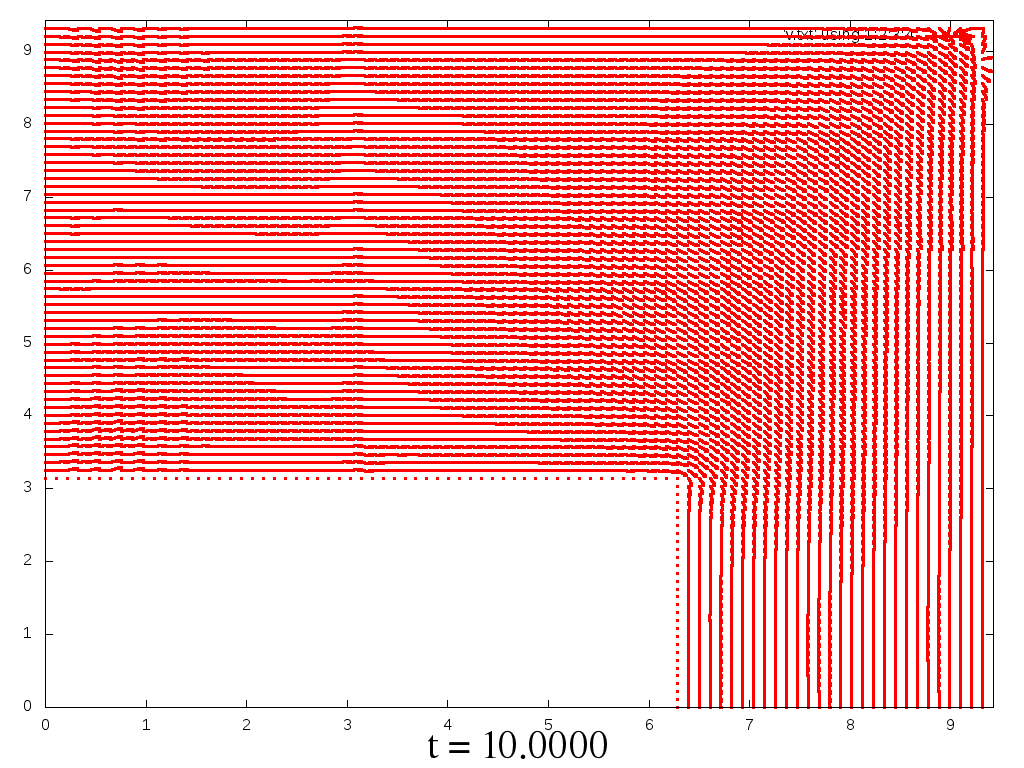
\includegraphics[width=1\linewidth]{./pics/0.1-30-50-51/v/10.png}}
\end{minipage}
\end{figure}

\begin{figure}[H]
\begin{minipage}[h]{0.43\linewidth}
\center{\includegraphics[width=1\linewidth]{./pics/0.1-30-50-51/v/20.png}}
\end{minipage}
\hfill
\begin{minipage}[h]{0.43\linewidth}
\center{\includegraphics[width=1\linewidth]{./pics/0.1-30-50-51/v/30.png}}
\end{minipage}
\end{figure}

\begin{figure}[H]
\begin{minipage}[h]{0.43\linewidth}
\center{\includegraphics[width=1\linewidth]{./pics/0.1-30-50-51/v/40.png}}
\end{minipage}
\hfill
\begin{minipage}[h]{0.43\linewidth}
\center{\includegraphics[width=1\linewidth]{./pics/0.1-30-50-51/v/50.png}}
\end{minipage}
\end{figure}

\begin{figure}[H]
\begin{minipage}[h]{0.43\linewidth}
\center{\includegraphics[width=1\linewidth]{./pics/0.1-30-50-51/g/0.png}}
\end{minipage}
\hfill
\begin{minipage}[h]{0.43\linewidth}
\center{\includegraphics[width=1\linewidth]{./pics/0.1-30-50-51/g/10.png}}
\end{minipage}
\end{figure}

\begin{figure}[H]
\begin{minipage}[h]{0.43\linewidth}
\center{\includegraphics[width=1\linewidth]{./pics/0.1-30-50-51/g/20.png}}
\end{minipage}
\hfill
\begin{minipage}[h]{0.43\linewidth}
\center{\includegraphics[width=1\linewidth]{./pics/0.1-30-50-51/g/30.png}}
\end{minipage}
\end{figure}

\begin{figure}[H]
\begin{minipage}[h]{0.43\linewidth}
\center{\includegraphics[width=1\linewidth]{./pics/0.1-30-50-51/g/40.png}}
\end{minipage}
\hfill
\begin{minipage}[h]{0.43\linewidth}
\center{\includegraphics[width=1\linewidth]{./pics/0.1-30-50-51/g/50.png}}
\end{minipage}
\end{figure}


%==================================================

\subsection{Графики для $\mu=0.01$} 
\subsubsection{$M_x=10$; $M_y=10$; $T=10$}
\begin{figure}[H]
\begin{minipage}[h]{0.43\linewidth}
\center{\includegraphics[width=1\linewidth]{./pics/0.01-10-10-21/v/0.png}}
\end{minipage}
\hfill
\begin{minipage}[h]{0.43\linewidth}
\center{\includegraphics[width=1\linewidth]{./pics/0.01-10-10-21/v/4.png}}
\end{minipage}
\end{figure}

\begin{figure}[H]
\begin{minipage}[h]{0.43\linewidth}
\center{\includegraphics[width=1\linewidth]{./pics/0.01-10-10-21/v/8.png}}
\end{minipage}
\hfill
\begin{minipage}[h]{0.43\linewidth}
\center{\includegraphics[width=1\linewidth]{./pics/0.01-10-10-21/v/12.png}}
\end{minipage}
\end{figure}

\begin{figure}[H]
\begin{minipage}[h]{0.43\linewidth}
\center{\includegraphics[width=1\linewidth]{./pics/0.01-10-10-21/v/16.png}}
\end{minipage}
\hfill
\begin{minipage}[h]{0.43\linewidth}
\center{\includegraphics[width=1\linewidth]{./pics/0.01-10-10-21/v/20.png}}
\end{minipage}
\end{figure}

\begin{figure}[H]
\begin{minipage}[h]{0.43\linewidth}
\center{\includegraphics[width=1\linewidth]{./pics/0.01-10-10-21/g/0.png}}
\end{minipage}
\hfill
\begin{minipage}[h]{0.43\linewidth}
\center{\includegraphics[width=1\linewidth]{./pics/0.01-10-10-21/g/4.png}}
\end{minipage}
\end{figure}

\begin{figure}[H]
\begin{minipage}[h]{0.43\linewidth}
\center{\includegraphics[width=1\linewidth]{./pics/0.01-10-10-21/g/8.png}}
\end{minipage}
\hfill
\begin{minipage}[h]{0.43\linewidth}
\center{\includegraphics[width=1\linewidth]{./pics/0.01-10-10-21/g/12.png}}
\end{minipage}
\end{figure}

\begin{figure}[H]
\begin{minipage}[h]{0.43\linewidth}
\center{\includegraphics[width=1\linewidth]{./pics/0.01-10-10-21/g/16.png}}
\end{minipage}
\hfill
\begin{minipage}[h]{0.43\linewidth}
\center{\includegraphics[width=1\linewidth]{./pics/0.01-10-10-21/g/20.png}}
\end{minipage}
\end{figure}


\subsubsection{$M_x=20$; $M_y=20$; $T=10$}
\begin{figure}[H]
\begin{minipage}[h]{0.43\linewidth}
\center{\includegraphics[width=1\linewidth]{./pics/0.01-20-10-21/v/0.png}}
\end{minipage}
\hfill
\begin{minipage}[h]{0.43\linewidth}
\center{\includegraphics[width=1\linewidth]{./pics/0.01-20-10-21/v/4.png}}
\end{minipage}
\end{figure}

\begin{figure}[H]
\begin{minipage}[h]{0.43\linewidth}
\center{\includegraphics[width=1\linewidth]{./pics/0.01-20-10-21/v/8.png}}
\end{minipage}
\hfill
\begin{minipage}[h]{0.43\linewidth}
\center{\includegraphics[width=1\linewidth]{./pics/0.01-20-10-21/v/12.png}}
\end{minipage}
\end{figure}

\begin{figure}[H]
\begin{minipage}[h]{0.43\linewidth}
\center{\includegraphics[width=1\linewidth]{./pics/0.01-20-10-21/v/16.png}}
\end{minipage}
\hfill
\begin{minipage}[h]{0.43\linewidth}
\center{\includegraphics[width=1\linewidth]{./pics/0.01-20-10-21/v/20.png}}
\end{minipage}
\end{figure}

\begin{figure}[H]
\begin{minipage}[h]{0.43\linewidth}
\center{\includegraphics[width=1\linewidth]{./pics/0.01-20-10-21/g/0.png}}
\end{minipage}
\hfill
\begin{minipage}[h]{0.43\linewidth}
\center{\includegraphics[width=1\linewidth]{./pics/0.01-20-10-21/g/4.png}}
\end{minipage}
\end{figure}

\begin{figure}[H]
\begin{minipage}[h]{0.43\linewidth}
\center{\includegraphics[width=1\linewidth]{./pics/0.01-20-10-21/g/8.png}}
\end{minipage}
\hfill
\begin{minipage}[h]{0.43\linewidth}
\center{\includegraphics[width=1\linewidth]{./pics/0.01-20-10-21/g/12.png}}
\end{minipage}
\end{figure}

\begin{figure}[H]
\begin{minipage}[h]{0.43\linewidth}
\center{\includegraphics[width=1\linewidth]{./pics/0.01-20-10-21/g/16.png}}
\end{minipage}
\hfill
\begin{minipage}[h]{0.43\linewidth}
\center{\includegraphics[width=1\linewidth]{./pics/0.01-20-10-21/g/20.png}}
\end{minipage}
\end{figure}



\subsubsection{$M_x=30$; $M_y=30$; $T=10$}
\begin{figure}[H]
\begin{minipage}[h]{0.43\linewidth}
\center{\includegraphics[width=1\linewidth]{./pics/0.01-30-10-21/v/0.png}}
\end{minipage}
\hfill
\begin{minipage}[h]{0.43\linewidth}
\center{\includegraphics[width=1\linewidth]{./pics/0.01-30-10-21/v/4.png}}
\end{minipage}
\end{figure}

\begin{figure}[H]
\begin{minipage}[h]{0.43\linewidth}
\center{\includegraphics[width=1\linewidth]{./pics/0.01-30-10-21/v/8.png}}
\end{minipage}
\hfill
\begin{minipage}[h]{0.43\linewidth}
\center{\includegraphics[width=1\linewidth]{./pics/0.01-30-10-21/v/12.png}}
\end{minipage}
\end{figure}

\begin{figure}[H]
\begin{minipage}[h]{0.43\linewidth}
\center{\includegraphics[width=1\linewidth]{./pics/0.01-30-10-21/v/16.png}}
\end{minipage}
\hfill
\begin{minipage}[h]{0.43\linewidth}
\center{\includegraphics[width=1\linewidth]{./pics/0.01-30-10-21/v/20.png}}
\end{minipage}
\end{figure}

\begin{figure}[H]
\begin{minipage}[h]{0.43\linewidth}
\center{\includegraphics[width=1\linewidth]{./pics/0.01-30-10-21/g/0.png}}
\end{minipage}
\hfill
\begin{minipage}[h]{0.43\linewidth}
\center{\includegraphics[width=1\linewidth]{./pics/0.01-30-10-21/g/4.png}}
\end{minipage}
\end{figure}

\begin{figure}[H]
\begin{minipage}[h]{0.43\linewidth}
\center{\includegraphics[width=1\linewidth]{./pics/0.01-30-10-21/g/8.png}}
\end{minipage}
\hfill
\begin{minipage}[h]{0.43\linewidth}
\center{\includegraphics[width=1\linewidth]{./pics/0.01-30-10-21/g/12.png}}
\end{minipage}
\end{figure}

\begin{figure}[H]
\begin{minipage}[h]{0.43\linewidth}
\center{\includegraphics[width=1\linewidth]{./pics/0.01-30-10-21/g/16.png}}
\end{minipage}
\hfill
\begin{minipage}[h]{0.43\linewidth}
\center{\includegraphics[width=1\linewidth]{./pics/0.01-30-10-21/g/20.png}}
\end{minipage}
\end{figure}



\subsubsection{$M_x=10$; $M_y=10$; $T=50$}
\begin{figure}[H]
\begin{minipage}[h]{0.43\linewidth}
\center{\includegraphics[width=1\linewidth]{./pics/0.01-10-50-51/v/0.png}}
\end{minipage}
\hfill
\begin{minipage}[h]{0.43\linewidth}
\center{\includegraphics[width=1\linewidth]{./pics/0.01-10-50-51/v/10.png}}
\end{minipage}
\end{figure}

\begin{figure}[H]
\begin{minipage}[h]{0.43\linewidth}
\center{\includegraphics[width=1\linewidth]{./pics/0.01-10-50-51/v/20.png}}
\end{minipage}
\hfill
\begin{minipage}[h]{0.43\linewidth}
\center{\includegraphics[width=1\linewidth]{./pics/0.01-10-50-51/v/30.png}}
\end{minipage}
\end{figure}

\begin{figure}[H]
\begin{minipage}[h]{0.43\linewidth}
\center{\includegraphics[width=1\linewidth]{./pics/0.01-10-50-51/v/40.png}}
\end{minipage}
\hfill
\begin{minipage}[h]{0.43\linewidth}
\center{\includegraphics[width=1\linewidth]{./pics/0.01-10-50-51/v/50.png}}
\end{minipage}
\end{figure}

\begin{figure}[H]
\begin{minipage}[h]{0.43\linewidth}
\center{\includegraphics[width=1\linewidth]{./pics/0.01-10-50-51/g/0.png}}
\end{minipage}
\hfill
\begin{minipage}[h]{0.43\linewidth}
\center{\includegraphics[width=1\linewidth]{./pics/0.01-10-50-51/g/10.png}}
\end{minipage}
\end{figure}

\begin{figure}[H]
\begin{minipage}[h]{0.43\linewidth}
\center{\includegraphics[width=1\linewidth]{./pics/0.01-10-50-51/g/20.png}}
\end{minipage}
\hfill
\begin{minipage}[h]{0.43\linewidth}
\center{\includegraphics[width=1\linewidth]{./pics/0.01-10-50-51/g/30.png}}
\end{minipage}
\end{figure}

\begin{figure}[H]
\begin{minipage}[h]{0.43\linewidth}
\center{\includegraphics[width=1\linewidth]{./pics/0.01-10-50-51/g/40.png}}
\end{minipage}
\hfill
\begin{minipage}[h]{0.43\linewidth}
\center{\includegraphics[width=1\linewidth]{./pics/0.01-10-50-51/g/50.png}}
\end{minipage}
\end{figure}


\subsubsection{$M_x=20$; $M_y=20$; $T=50$}
\begin{figure}[H]
\begin{minipage}[h]{0.43\linewidth}
\center{\includegraphics[width=1\linewidth]{./pics/0.01-20-50-51/v/0.png}}
\end{minipage}
\hfill
\begin{minipage}[h]{0.43\linewidth}
\center{\includegraphics[width=1\linewidth]{./pics/0.01-20-50-51/v/10.png}}
\end{minipage}
\end{figure}

\begin{figure}[H]
\begin{minipage}[h]{0.43\linewidth}
\center{\includegraphics[width=1\linewidth]{./pics/0.01-20-50-51/v/20.png}}
\end{minipage}
\hfill
\begin{minipage}[h]{0.43\linewidth}
\center{\includegraphics[width=1\linewidth]{./pics/0.01-20-50-51/v/30.png}}
\end{minipage}
\end{figure}

\begin{figure}[H]
\begin{minipage}[h]{0.43\linewidth}
\center{\includegraphics[width=1\linewidth]{./pics/0.01-20-50-51/v/40.png}}
\end{minipage}
\hfill
\begin{minipage}[h]{0.43\linewidth}
\center{\includegraphics[width=1\linewidth]{./pics/0.01-20-50-51/v/50.png}}
\end{minipage}
\end{figure}

\begin{figure}[H]
\begin{minipage}[h]{0.43\linewidth}
\center{\includegraphics[width=1\linewidth]{./pics/0.01-20-50-51/g/0.png}}
\end{minipage}
\hfill
\begin{minipage}[h]{0.43\linewidth}
\center{\includegraphics[width=1\linewidth]{./pics/0.01-20-50-51/g/10.png}}
\end{minipage}
\end{figure}

\begin{figure}[H]
\begin{minipage}[h]{0.43\linewidth}
\center{\includegraphics[width=1\linewidth]{./pics/0.01-20-50-51/g/20.png}}
\end{minipage}
\hfill
\begin{minipage}[h]{0.43\linewidth}
\center{\includegraphics[width=1\linewidth]{./pics/0.01-20-50-51/g/30.png}}
\end{minipage}
\end{figure}

\begin{figure}[H]
\begin{minipage}[h]{0.43\linewidth}
\center{\includegraphics[width=1\linewidth]{./pics/0.01-20-50-51/g/40.png}}
\end{minipage}
\hfill
\begin{minipage}[h]{0.43\linewidth}
\center{\includegraphics[width=1\linewidth]{./pics/0.01-20-50-51/g/50.png}}
\end{minipage}
\end{figure}



\subsubsection{$M_x=30$; $M_y=30$; $T=50$}
\begin{figure}[H]
\begin{minipage}[h]{0.43\linewidth}
\center{\includegraphics[width=1\linewidth]{./pics/0.01-30-50-51/v/0.png}}
\end{minipage}
\hfill
\begin{minipage}[h]{0.43\linewidth}
\center{\includegraphics[width=1\linewidth]{./pics/0.01-30-50-51/v/10.png}}
\end{minipage}
\end{figure}

\begin{figure}[H]
\begin{minipage}[h]{0.43\linewidth}
\center{\includegraphics[width=1\linewidth]{./pics/0.01-30-50-51/v/20.png}}
\end{minipage}
\hfill
\begin{minipage}[h]{0.43\linewidth}
\center{\includegraphics[width=1\linewidth]{./pics/0.01-30-50-51/v/30.png}}
\end{minipage}
\end{figure}

\begin{figure}[H]
\begin{minipage}[h]{0.43\linewidth}
\center{\includegraphics[width=1\linewidth]{./pics/0.01-30-50-51/v/40.png}}
\end{minipage}
\hfill
\begin{minipage}[h]{0.43\linewidth}
\center{\includegraphics[width=1\linewidth]{./pics/0.01-30-50-51/v/50.png}}
\end{minipage}
\end{figure}

\begin{figure}[H]
\begin{minipage}[h]{0.43\linewidth}
\center{\includegraphics[width=1\linewidth]{./pics/0.01-30-50-51/g/0.png}}
\end{minipage}
\hfill
\begin{minipage}[h]{0.43\linewidth}
\center{\includegraphics[width=1\linewidth]{./pics/0.01-30-50-51/g/10.png}}
\end{minipage}
\end{figure}

\begin{figure}[H]
\begin{minipage}[h]{0.43\linewidth}
\center{\includegraphics[width=1\linewidth]{./pics/0.01-30-50-51/g/20.png}}
\end{minipage}
\hfill
\begin{minipage}[h]{0.43\linewidth}
\center{\includegraphics[width=1\linewidth]{./pics/0.01-30-50-51/g/30.png}}
\end{minipage}
\end{figure}

\begin{figure}[H]
\begin{minipage}[h]{0.43\linewidth}
\center{\includegraphics[width=1\linewidth]{./pics/0.01-30-50-51/g/40.png}}
\end{minipage}
\hfill
\begin{minipage}[h]{0.43\linewidth}
\center{\includegraphics[width=1\linewidth]{./pics/0.01-30-50-51/g/50.png}}
\end{minipage}
\end{figure}


%================================================================

\subsection{Графики для $\mu=0.001$} 
\subsubsection{$M_x=10$; $M_y=10$; $T=10$}
\begin{figure}[H]
\begin{minipage}[h]{0.43\linewidth}
\center{\includegraphics[width=1\linewidth]{./pics/0.001-10-10-21/v/0.png}}
\end{minipage}
\hfill
\begin{minipage}[h]{0.43\linewidth}
\center{\includegraphics[width=1\linewidth]{./pics/0.001-10-10-21/v/4.png}}
\end{minipage}
\end{figure}

\begin{figure}[H]
\begin{minipage}[h]{0.43\linewidth}
\center{\includegraphics[width=1\linewidth]{./pics/0.001-10-10-21/v/8.png}}
\end{minipage}
\hfill
\begin{minipage}[h]{0.43\linewidth}
\center{\includegraphics[width=1\linewidth]{./pics/0.001-10-10-21/v/12.png}}
\end{minipage}
\end{figure}

\begin{figure}[H]
\begin{minipage}[h]{0.43\linewidth}
\center{\includegraphics[width=1\linewidth]{./pics/0.001-10-10-21/v/16.png}}
\end{minipage}
\hfill
\begin{minipage}[h]{0.43\linewidth}
\center{\includegraphics[width=1\linewidth]{./pics/0.001-10-10-21/v/20.png}}
\end{minipage}
\end{figure}

\begin{figure}[H]
\begin{minipage}[h]{0.43\linewidth}
\center{\includegraphics[width=1\linewidth]{./pics/0.001-10-10-21/g/0.png}}
\end{minipage}
\hfill
\begin{minipage}[h]{0.43\linewidth}
\center{\includegraphics[width=1\linewidth]{./pics/0.001-10-10-21/g/4.png}}
\end{minipage}
\end{figure}

\begin{figure}[H]
\begin{minipage}[h]{0.43\linewidth}
\center{\includegraphics[width=1\linewidth]{./pics/0.001-10-10-21/g/8.png}}
\end{minipage}
\hfill
\begin{minipage}[h]{0.43\linewidth}
\center{\includegraphics[width=1\linewidth]{./pics/0.001-10-10-21/g/12.png}}
\end{minipage}
\end{figure}

\begin{figure}[H]
\begin{minipage}[h]{0.43\linewidth}
\center{\includegraphics[width=1\linewidth]{./pics/0.001-10-10-21/g/16.png}}
\end{minipage}
\hfill
\begin{minipage}[h]{0.43\linewidth}
\center{\includegraphics[width=1\linewidth]{./pics/0.001-10-10-21/g/20.png}}
\end{minipage}
\end{figure}


\subsubsection{$M_x=20$; $M_y=20$; $T=10$}
\begin{figure}[H]
\begin{minipage}[h]{0.43\linewidth}
\center{\includegraphics[width=1\linewidth]{./pics/0.001-20-10-21/v/0.png}}
\end{minipage}
\hfill
\begin{minipage}[h]{0.43\linewidth}
\center{\includegraphics[width=1\linewidth]{./pics/0.001-20-10-21/v/4.png}}
\end{minipage}
\end{figure}

\begin{figure}[H]
\begin{minipage}[h]{0.43\linewidth}
\center{\includegraphics[width=1\linewidth]{./pics/0.001-20-10-21/v/8.png}}
\end{minipage}
\hfill
\begin{minipage}[h]{0.43\linewidth}
\center{\includegraphics[width=1\linewidth]{./pics/0.001-20-10-21/v/12.png}}
\end{minipage}
\end{figure}

\begin{figure}[H]
\begin{minipage}[h]{0.43\linewidth}
\center{\includegraphics[width=1\linewidth]{./pics/0.001-20-10-21/v/16.png}}
\end{minipage}
\hfill
\begin{minipage}[h]{0.43\linewidth}
\center{\includegraphics[width=1\linewidth]{./pics/0.001-20-10-21/v/20.png}}
\end{minipage}
\end{figure}

\begin{figure}[H]
\begin{minipage}[h]{0.43\linewidth}
\center{\includegraphics[width=1\linewidth]{./pics/0.001-20-10-21/g/0.png}}
\end{minipage}
\hfill
\begin{minipage}[h]{0.43\linewidth}
\center{\includegraphics[width=1\linewidth]{./pics/0.001-20-10-21/g/4.png}}
\end{minipage}
\end{figure}

\begin{figure}[H]
\begin{minipage}[h]{0.43\linewidth}
\center{\includegraphics[width=1\linewidth]{./pics/0.001-20-10-21/g/8.png}}
\end{minipage}
\hfill
\begin{minipage}[h]{0.43\linewidth}
\center{\includegraphics[width=1\linewidth]{./pics/0.001-20-10-21/g/12.png}}
\end{minipage}
\end{figure}

\begin{figure}[H]
\begin{minipage}[h]{0.43\linewidth}
\center{\includegraphics[width=1\linewidth]{./pics/0.001-20-10-21/g/16.png}}
\end{minipage}
\hfill
\begin{minipage}[h]{0.43\linewidth}
\center{\includegraphics[width=1\linewidth]{./pics/0.001-20-10-21/g/20.png}}
\end{minipage}
\end{figure}



\subsubsection{$M_x=30$; $M_y=30$; $T=10$}
\begin{figure}[H]
\begin{minipage}[h]{0.43\linewidth}
\center{\includegraphics[width=1\linewidth]{./pics/0.001-30-10-21/v/0.png}}
\end{minipage}
\hfill
\begin{minipage}[h]{0.43\linewidth}
\center{\includegraphics[width=1\linewidth]{./pics/0.001-30-10-21/v/4.png}}
\end{minipage}
\end{figure}

\begin{figure}[H]
\begin{minipage}[h]{0.43\linewidth}
\center{\includegraphics[width=1\linewidth]{./pics/0.001-30-10-21/v/8.png}}
\end{minipage}
\hfill
\begin{minipage}[h]{0.43\linewidth}
\center{\includegraphics[width=1\linewidth]{./pics/0.001-30-10-21/v/12.png}}
\end{minipage}
\end{figure}

\begin{figure}[H]
\begin{minipage}[h]{0.43\linewidth}
\center{\includegraphics[width=1\linewidth]{./pics/0.001-30-10-21/v/16.png}}
\end{minipage}
\hfill
\begin{minipage}[h]{0.43\linewidth}
\center{\includegraphics[width=1\linewidth]{./pics/0.001-30-10-21/v/20.png}}
\end{minipage}
\end{figure}

\begin{figure}[H]
\begin{minipage}[h]{0.43\linewidth}
\center{\includegraphics[width=1\linewidth]{./pics/0.001-30-10-21/g/0.png}}
\end{minipage}
\hfill
\begin{minipage}[h]{0.43\linewidth}
\center{\includegraphics[width=1\linewidth]{./pics/0.001-30-10-21/g/4.png}}
\end{minipage}
\end{figure}

\begin{figure}[H]
\begin{minipage}[h]{0.43\linewidth}
\center{\includegraphics[width=1\linewidth]{./pics/0.001-30-10-21/g/8.png}}
\end{minipage}
\hfill
\begin{minipage}[h]{0.43\linewidth}
\center{\includegraphics[width=1\linewidth]{./pics/0.001-30-10-21/g/12.png}}
\end{minipage}
\end{figure}

\begin{figure}[H]
\begin{minipage}[h]{0.43\linewidth}
\center{\includegraphics[width=1\linewidth]{./pics/0.001-30-10-21/g/16.png}}
\end{minipage}
\hfill
\begin{minipage}[h]{0.43\linewidth}
\center{\includegraphics[width=1\linewidth]{./pics/0.001-30-10-21/g/20.png}}
\end{minipage}
\end{figure}



\subsubsection{$M_x=10$; $M_y=10$; $T=50$}
\begin{figure}[H]
\begin{minipage}[h]{0.43\linewidth}
\center{\includegraphics[width=1\linewidth]{./pics/0.001-10-50-51/v/0.png}}
\end{minipage}
\hfill
\begin{minipage}[h]{0.43\linewidth}
\center{\includegraphics[width=1\linewidth]{./pics/0.001-10-50-51/v/10.png}}
\end{minipage}
\end{figure}

\begin{figure}[H]
\begin{minipage}[h]{0.43\linewidth}
\center{\includegraphics[width=1\linewidth]{./pics/0.001-10-50-51/v/20.png}}
\end{minipage}
\hfill
\begin{minipage}[h]{0.43\linewidth}
\center{\includegraphics[width=1\linewidth]{./pics/0.001-10-50-51/v/30.png}}
\end{minipage}
\end{figure}

\begin{figure}[H]
\begin{minipage}[h]{0.43\linewidth}
\center{\includegraphics[width=1\linewidth]{./pics/0.001-10-50-51/v/40.png}}
\end{minipage}
\hfill
\begin{minipage}[h]{0.43\linewidth}
\center{\includegraphics[width=1\linewidth]{./pics/0.001-10-50-51/v/50.png}}
\end{minipage}
\end{figure}

\begin{figure}[H]
\begin{minipage}[h]{0.43\linewidth}
\center{\includegraphics[width=1\linewidth]{./pics/0.001-10-50-51/g/0.png}}
\end{minipage}
\hfill
\begin{minipage}[h]{0.43\linewidth}
\center{\includegraphics[width=1\linewidth]{./pics/0.001-10-50-51/g/10.png}}
\end{minipage}
\end{figure}

\begin{figure}[H]
\begin{minipage}[h]{0.43\linewidth}
\center{\includegraphics[width=1\linewidth]{./pics/0.001-10-50-51/g/20.png}}
\end{minipage}
\hfill
\begin{minipage}[h]{0.43\linewidth}
\center{\includegraphics[width=1\linewidth]{./pics/0.001-10-50-51/g/30.png}}
\end{minipage}
\end{figure}

\begin{figure}[H]
\begin{minipage}[h]{0.43\linewidth}
\center{\includegraphics[width=1\linewidth]{./pics/0.001-10-50-51/g/40.png}}
\end{minipage}
\hfill
\begin{minipage}[h]{0.43\linewidth}
\center{\includegraphics[width=1\linewidth]{./pics/0.001-10-50-51/g/50.png}}
\end{minipage}
\end{figure}


\subsubsection{$M_x=20$; $M_y=20$; $T=50$}
\begin{figure}[H]
\begin{minipage}[h]{0.43\linewidth}
\center{\includegraphics[width=1\linewidth]{./pics/0.001-20-50-51/v/0.png}}
\end{minipage}
\hfill
\begin{minipage}[h]{0.43\linewidth}
\center{\includegraphics[width=1\linewidth]{./pics/0.001-20-50-51/v/10.png}}
\end{minipage}
\end{figure}

\begin{figure}[H]
\begin{minipage}[h]{0.43\linewidth}
\center{\includegraphics[width=1\linewidth]{./pics/0.001-20-50-51/v/20.png}}
\end{minipage}
\hfill
\begin{minipage}[h]{0.43\linewidth}
\center{\includegraphics[width=1\linewidth]{./pics/0.001-20-50-51/v/30.png}}
\end{minipage}
\end{figure}

\begin{figure}[H]
\begin{minipage}[h]{0.43\linewidth}
\center{\includegraphics[width=1\linewidth]{./pics/0.001-20-50-51/v/40.png}}
\end{minipage}
\hfill
\begin{minipage}[h]{0.43\linewidth}
\center{\includegraphics[width=1\linewidth]{./pics/0.001-20-50-51/v/50.png}}
\end{minipage}
\end{figure}

\begin{figure}[H]
\begin{minipage}[h]{0.43\linewidth}
\center{\includegraphics[width=1\linewidth]{./pics/0.001-20-50-51/g/0.png}}
\end{minipage}
\hfill
\begin{minipage}[h]{0.43\linewidth}
\center{\includegraphics[width=1\linewidth]{./pics/0.001-20-50-51/g/10.png}}
\end{minipage}
\end{figure}

\begin{figure}[H]
\begin{minipage}[h]{0.43\linewidth}
\center{\includegraphics[width=1\linewidth]{./pics/0.001-20-50-51/g/20.png}}
\end{minipage}
\hfill
\begin{minipage}[h]{0.43\linewidth}
\center{\includegraphics[width=1\linewidth]{./pics/0.001-20-50-51/g/30.png}}
\end{minipage}
\end{figure}

\begin{figure}[H]
\begin{minipage}[h]{0.43\linewidth}
\center{\includegraphics[width=1\linewidth]{./pics/0.001-20-50-51/g/40.png}}
\end{minipage}
\hfill
\begin{minipage}[h]{0.43\linewidth}
\center{\includegraphics[width=1\linewidth]{./pics/0.001-20-50-51/g/50.png}}
\end{minipage}
\end{figure}



\subsubsection{$M_x=30$; $M_y=30$; $T=50$}
\begin{figure}[H]
\begin{minipage}[h]{0.43\linewidth}
\center{\includegraphics[width=1\linewidth]{./pics/0.001-30-50-51/v/0.png}}
\end{minipage}
\hfill
\begin{minipage}[h]{0.43\linewidth}
\center{\includegraphics[width=1\linewidth]{./pics/0.001-30-50-51/v/10.png}}
\end{minipage}
\end{figure}

\begin{figure}[H]
\begin{minipage}[h]{0.43\linewidth}
\center{\includegraphics[width=1\linewidth]{./pics/0.001-30-50-51/v/20.png}}
\end{minipage}
\hfill
\begin{minipage}[h]{0.43\linewidth}
\center{\includegraphics[width=1\linewidth]{./pics/0.001-30-50-51/v/30.png}}
\end{minipage}
\end{figure}

\begin{figure}[H]
\begin{minipage}[h]{0.43\linewidth}
\center{\includegraphics[width=1\linewidth]{./pics/0.001-30-50-51/v/40.png}}
\end{minipage}
\hfill
\begin{minipage}[h]{0.43\linewidth}
\center{\includegraphics[width=1\linewidth]{./pics/0.001-30-50-51/v/50.png}}
\end{minipage}
\end{figure}

\begin{figure}[H]
\begin{minipage}[h]{0.43\linewidth}
\center{\includegraphics[width=1\linewidth]{./pics/0.001-30-50-51/g/0.png}}
\end{minipage}
\hfill
\begin{minipage}[h]{0.43\linewidth}
\center{\includegraphics[width=1\linewidth]{./pics/0.001-30-50-51/g/10.png}}
\end{minipage}
\end{figure}

\begin{figure}[H]
\begin{minipage}[h]{0.43\linewidth}
\center{\includegraphics[width=1\linewidth]{./pics/0.001-30-50-51/g/20.png}}
\end{minipage}
\hfill
\begin{minipage}[h]{0.43\linewidth}
\center{\includegraphics[width=1\linewidth]{./pics/0.001-30-50-51/g/30.png}}
\end{minipage}
\end{figure}

\begin{figure}[H]
\begin{minipage}[h]{0.43\linewidth}
\center{\includegraphics[width=1\linewidth]{./pics/0.001-30-50-51/g/40.png}}
\end{minipage}
\hfill
\begin{minipage}[h]{0.43\linewidth}
\center{\includegraphics[width=1\linewidth]{./pics/0.001-30-50-51/g/50.png}}
\end{minipage}
\end{figure}



%\include{./2_scheme_results}

\end {document}
